% Монгол улсын дугаар таних — явцын тайлан (XeLaTeX / Tectonic)
\documentclass[12pt,a4paper,oneside]{report}
\usepackage{fontspec}
\setmainfont{Liberation Serif}
\setsansfont{Liberation Sans}
\setmonofont{Liberation Mono}[Scale=0.85]
\usepackage{polyglossia}
\setmainlanguage{mongolian}
\usepackage[a4paper,top=2.5cm,bottom=2.5cm,left=3cm,right=2cm]{geometry}
\usepackage{setspace}\onehalfspacing
\usepackage{graphicx,booktabs,array,multirow,longtable,float,caption,subcaption,amsmath,amssymb,xcolor,enumitem,listings,tocloft,titlesec,fancyhdr,url}
\usepackage[hidelinks]{hyperref}
\graphicspath{{figures/}}
\setlist{nosep}
% ---------- editable fields ----------
\newcommand{\univ}{МОНГОЛ УЛСЫН ИХ СУРГУУЛЬ}
\newcommand{\school}{МЭДЭЭЛЛИЙН ТЕХНОЛОГИ, ЭЛЕКТРОНИКИЙН СУРГУУЛЬ}
\newcommand{\dept}{МЭДЭЭЛЭЛ, КОМПЬЮТЕРЫН УХААНЫ ТЭНХИМ}
\newcommand{\studentname}{[Овгийн эхний үсэг]. [Нэр]}
\newcommand{\studentid}{[Оюутны код]}
\newcommand{\supervisor}{[Удирдагчийн нэр]}
\newcommand{\cosupervisor}{[Хамтран удирдагчийн нэр]}
\newcommand{\program}{Мэдээллийн технологи (D061303)}
\newcommand{\reporttype}{Бакалаврын судалгааны ажил, Явцын тайлан}
\newcommand{\titlemn}{ЗОГСООЛЫН СИСТЕМД ЗОРИУЛСАН МОНГОЛ УЛСЫН ДУГААР ТАНИХ ГҮН СУРГАЛТЫН ЗАГВАР БҮТЭЭХ}
\newcommand{\titleen}{(Developing a Deep Learning Model for Mongolian License Plate Recognition for Parking Systems)}
\newcommand{\reportdate}{2026 оны 10 дугаар сар}
% ---------- styling ----------
\titleformat{\chapter}[hang]{\bfseries\LARGE}{\thechapter.}{0.6em}{\MakeUppercase}
\titlespacing*{\chapter}{0pt}{0pt}{20pt}
\titleformat{\section}{\bfseries\large}{\thesection}{0.8em}{}
\titleformat{\subsection}{\bfseries\normalsize}{\thesubsection}{0.8em}{}
\gappto\captionsmongolian{\renewcommand{\contentsname}{ГАРЧИГ}\renewcommand{\listfigurename}{ЗУРГИЙН ЖАГСААЛТ}\renewcommand{\listtablename}{ХҮСНЭГТИЙН ЖАГСААЛТ}\renewcommand{\figurename}{Зураг}\renewcommand{\tablename}{Хүснэгт}\renewcommand{\bibname}{НОМ ЗҮЙ}\renewcommand{\appendixname}{Хавсралт}\renewcommand{\chaptername}{Бүлэг}\renewcommand{\lstlistingname}{Код}}
\captionsetup{labelfont=bf,labelsep=period,font=small,justification=justified}
\renewcommand{\cftchapfont}{\normalfont}\renewcommand{\cftchappagefont}{\normalfont}\renewcommand{\cftchapleader}{\cftdotfill{\cftdotsep}}
\renewcommand{\cfttoctitlefont}{\hfill\normalsize\bfseries}\renewcommand{\cftaftertoctitle}{\hfill}
\renewcommand{\cftloftitlefont}{\hfill\normalsize\bfseries}\renewcommand{\cftafterloftitle}{\hfill}
\renewcommand{\cftlottitlefont}{\hfill\normalsize\bfseries}\renewcommand{\cftafterlottitle}{\hfill}
\pagestyle{fancy}\fancyhf{}\fancyhead[L]{\itshape\small\leftmark}\fancyfoot[C]{\thepage}\renewcommand{\headrulewidth}{0pt}
\renewcommand{\chaptermark}[1]{\markboth{БҮЛЭГ \thechapter.\ #1}{}}
\lstset{basicstyle=\ttfamily\footnotesize,breaklines=true,frame=single,columns=fullflexible,keepspaces=true,showstringspaces=false,numbers=left,numberstyle=\tiny,xleftmargin=2em}
\newcommand{\plate}[1]{\texttt{#1}}
\begin{document}
% ================= НҮҮР 1 =================
\begin{titlepage}\centering
{\bfseries\small \univ\\ \school\\ \dept\par}
\vspace{3.5cm}
{\large \studentname\par}
\vspace{3cm}
{\bfseries\Large \titlemn\par}\vspace{0.4cm}
{\bfseries\large \titleen\par}\vspace{0.8cm}
{\program\\ \reporttype\par}
\vfill
{Улаанбаатар\\[0.4cm] \reportdate\par}
\end{titlepage}
% ================= НҮҮР 2 =================
\begin{titlepage}\centering
{\bfseries\small \univ\\ \school\\ \dept\par}
\vspace{5cm}
{\bfseries\Large \titlemn\par}\vspace{0.4cm}
{\bfseries\large \titleen\par}\vspace{0.8cm}
{\program\\ \reporttype\par}
\vspace{3cm}
\begin{tabular}{p{3.8cm}p{4.3cm}p{6.5cm}}
Удирдагч: & \rule{4cm}{0.4pt} & \supervisor\\[0.6cm]
Хамтран удирдагч: & \rule{4cm}{0.4pt} & \cosupervisor\\[0.6cm]
Гүйцэтгэсэн: & \rule{4cm}{0.4pt} & \studentname\ (\studentid)\\
\end{tabular}
\vfill
{Улаанбаатар\\[0.4cm] \reportdate\par}
\end{titlepage}
% ================= ТӨЛӨВЛӨГӨӨ =================
\thispagestyle{empty}\vspace*{\fill}\begin{center}{\bfseries\Large ҮЕЧИЛСЭН ТӨЛӨВЛӨГӨӨ}\\[1em]
Энэ хуудасны оронд тамгалагдсан үечилсэн төлөвлөгөөг хавсаргана.\\(Скан хийсэн файлаа \texttt{figures/plan.pdf} нэрээр хуулж \texttt{main.tex}-д \texttt{includepdf} хийнэ.)\end{center}\vspace*{\fill}\clearpage
% ================= БАТАЛГАА =================
\pagenumbering{roman}\setcounter{page}{2}
\chapter*{Зохиогчийн баталгаа}
Миний бие \studentname\ «\titlemn» сэдэвтэй судалгааны ажлыг гүйцэтгэсэн болохыг зарлаж дараах зүйлсийг баталж байна:
\begin{itemize}[leftmargin=2em]
\item Ажил нь бүхэлдээ Монгол Улсын Их Сургуульд дээд боловсролын зэрэг горилохоор дэвшүүлсэн болно.
\item Энэ ажлын аль нэг хэсгийг эсвэл бүхлээр нь ямар нэг их, дээд сургуулийн зэрэг горилохоор оруулж байгаагүй болно.
\item Бусдын хийсэн ажлаас хуулбарлаагүй, эшлэл, зүүлтийг зохистой хийсэн болно.
\item Ажлыг зохиогч би хийсэн ба миний хийсэн ажил, бусдын дэмжлэгийг ажилд тодорхой тусгасан болно.
\item Ажилд тусалсан бүх эх сурвалжид талархаж байна.
\end{itemize}
\vspace{1em}Гарын үсэг: \rule{5cm}{0.4pt}\\[0.6em] Огноо: \rule{3cm}{0.4pt}
\clearpage
\tableofcontents\clearpage
\listoffigures\clearpage
\listoftables\clearpage
\pagenumbering{arabic}
\chapter*{УДИРТГАЛ}\addcontentsline{toc}{chapter}{УДИРТГАЛ}\markboth{УДИРТГАЛ}{}
\textbf{Сэдвийн үндэслэл.} Улаанбаатар хотод бүртгэлтэй тээврийн хэрэгслийн тоо 2025 оны байдлаар 730 мянгаар хязгаарлагдах шийдвэр гарсан бөгөөд зогсоолын хүрэлцээ, төлбөрийн автоматжуулалт нь хотын дэд бүтцийн тулгамдсан асуудлын нэг болоод байна~\cite{asianews2025}. Зогсоолын хаалгыг автоматаар нээх, төлбөрийг машины дугаараар тооцох, орох-гарах үйл явдлыг тасалбаргүйгээр тулгах зэрэг үйлдлийн суурь нь улсын дугаарыг камерын кадраас автоматаар таних (Automatic License Plate Recognition, ALPR) технологи юм. Олон улсын арилжааны ALPR шийдлүүд нь латин цагаан толгой эсвэл хятад дугаарт тохируулагдсан бол Монгол улсын дугаар нь орос цагаан толгойд байдаггүй Ө, Ү үсэг бүхий монгол кирилл үсгээр бичигддэг, нэг мөрт ба хоёр мөрт гэсэн хоёр физик хэлбэртэй~\cite{wikimn}. Иймээс бэлэн OCR загварууд монгол дугаарыг шууд уншиж чаддаггүй, дугаарын дүрмийг мэддэггүй тул латин--кирилл ижил хэлбэрт үсгийг андуурдаг.

\textbf{Сэдвийг сонгосон шалтгаан.} Нэгдүгээрт, монгол дугаарт зориулсан нээлттэй, текстээр шошголсон өгөгдлийн сан, хэвлэгдсэн судалгааны ажил байхгүй тул өгөгдлийг нэгтгэх, үнэлгээний протокол тогтоох нь өөрөө шинэлэг. Хоёрдугаарт, YOLO~\cite{yolo11} хэмээх хөнгөн илрүүлэгч, CRNN+CTC~\cite{shi2017crnn,graves2006ctc} дарааллын уншигч зэрэг сүүлийн үеийн загварууд нь нэг кадрыг хэдхэн миллисекундэд боловсруулж чадах болсноор зогсоолын хаалга дээр бодит цагт ажиллах боломж бүрдсэн. Гуравдугаарт, нэг кадрын алдааг олон кадрын саналаар засах арга нь видео ALPR-д 10--15 нэгж хувийн ахиц өгдөг нь судалгаагаар батлагдсан~\cite{laroca2018,wang2026mt} тул үүнийг монгол дугаарт хэрэгжүүлэх нь практик ач холбогдолтой.

\textbf{Судалгааны зорилго.} Зогсоолын системийн мэдрэхүйн модуль болох, Монгол улсын дугаарыг камерын кадраас 95 хувиас дээш бүрэн зөв уншдаг, нэг кадрыг 100 миллисекундээс бага хугацаанд боловсруулдаг, олон кадраар баталгаажуулдаг гүн сургалтын загвар бүтээхэд оршино.

\textbf{Судалгааны зорилтууд.} Зорилгод хүрэхийн тулд дараах зорилтуудыг дэвшүүлэв:
\begin{enumerate}[leftmargin=2.5em]
\item Дугаар таних олон улсын судалгаа, монгол дугаарын бүтэц, нээлттэй өгөгдлийн эх үүсвэрүүдийг судалж, цөөн өгөгдөлтэй нөхцөлд тохирох хандлагыг сонгох;
\item Олдсон бүх эх үүсвэрийг (GitHub, Roboflow, HuggingFace, MLUB тэмцээн) нэгтгэж, тэмдэгтийн хайрцгаас дугаарын текст сэргээх, дугаарын давхцалгүй хуваалт хийх, синтетик дугаар үүсгэх боловсруулалтын урсгал бүтээх;
\item YOLO11n дугаар илрүүлэгчийг хоёр үе шаттай сургаж mAP$_{50}\ge0.95$-д хүргэх;
\item Монгол кирилл үсгийн бүрэн олонлог дээр CRNN+CTC уншигчийг синтетик ба бодит өгөгдлөөр үе шаттай сургаж, нэг ба хоёр мөрт дугаарыг хоёуланг нь уншдаг болгох;
\item Дугаарын дүрэм, аймгийн кодын хүснэгт болон итгэлээр жинлэсэн тэмдэгт тус бүрийн саналд суурилсан олон кадрын баталгаажуулалт хэрэгжүүлэх;
\item Үр дүнг хэмжүүрээр (mAP, бүтэн дугаарын нарийвчлал, CER, хугацаа) үнэлж, алдааны шинжилгээ хийж, туршилтын интерфэйс бүтээн, дараагийн шатны ажлыг тодорхойлох.
\end{enumerate}

\textbf{Судалгааны хүрээ.} Энэ тайланд тусгасан ажил нь зогсож буй эсвэл удаан хөдөлж буй тээврийн хэрэгслийн дугаарыг өдрийн гэрэлд таних асуудалд хамаарна. Зогсоолын бүрэн систем (орох-гарах бүртгэлийн сан, төлбөр, хаалганы удирдлага) болон шөнийн, цас борооны нөхцөл дараагийн шатанд хамаарна. Дипломат (улаан, ДК), цэргийн, чиргүүлийн тусгай дугаар энэ ажилд ороогүй.

\textbf{Явцын байдал.} Ажлыг 2026 оны 10 дугаар сарын 14-нд эхлүүлж, нээлттэй эх үүсвэрээс 68 бүтэн дүрстэй зураг, 7392 бодит дугаарын тайралт, 8823 олон улсын зураг, 3 бичлэг цуглуулж, 90\,021 синтетик мөр зураг үүсгэв. Илрүүлэгч монгол шалгалтын олонлог дээр mAP$_{50}=0.992$, уншигч 1491 бодит дугаар дээр 96.8 хувийн бүрэн зөв уншилт (CER 0.65 хувь), бүхэл урсгал нэг 1080p кадрыг 7.3~мс-д боловсруулж байна. Бүтэн дүрстэй 19 дугаарын жижиг тест дээр төгсгөл хүртэлх нарийвчлал 73.7 хувь (9 кадрын саналаар 78.9 хувь) байгаа нь домэйн зөрүү ба ховор үсгийн асуудлыг илтгэж байгааг 5 дугаар бүлэгт хэлэлцэв.

\textbf{Тайлангийн бүтэц.} 1 дүгээр бүлэгт дугаар таних судалгааны тойм, 2 дугаар бүлэгт өгөгдлийн эх үүсвэр, боловсруулалт, синтетик үүсгэлт, 3 дугаар бүлэгт таних системийн арга зүй ба сургалтын тохиргоо, 4 дүгээр бүлэгт туршилт, үр дүн, алдааны шинжилгээ, 5 дугаар бүлэгт хэлэлцүүлэг, хязгаарлалт, цаашдын ажлыг тус тус тусгав.

\chapter{ДУГААР ТАНИХ СУДАЛГААНЫ ТОЙМ БА ОНОЛЫН ҮНДЭС}
\section{Асуудлын ангилал ба хоёр шатлалт хандлага}
Улсын дугаар таних асуудлыг уламжлалт байдлаар (1) дугаарын байрлалыг олох (plate detection), (2) дугаарын тэмдэгтүүдийг унших (plate recognition) гэсэн хоёр шатанд хуваадаг~\cite{laroca2018}. Эрт үеийн системүүд өнгө, ирмэг, морфологи дээр суурилсан дүрэмт аргаар дугаарыг олж, тэмдэгт тус бүрийг сегментчилээд ангилагчаар таньдаг байсан бол гүн сургалтын үед илрүүлэлтийг нэг шатлалт детектор (YOLO, SSD), уншилтыг сегментчлэлгүй дарааллын загвар (CRNN+CTC, attention-based) гүйцэтгэх болсон. Сегментчлэлгүй уншилт нь бохир, бүдэг, налуу дугаарт тэмдэгт тус бүрийг салгах шаардлагагүй тул илүү тэсвэртэй.

\section{Нэг шатлалт илрүүлэгч: YOLO гэр бүл}
YOLO (You Only Look Once) нь зургийг нэг удаа сүлжээгээр нэвтрүүлж объектын хайрцаг, ангийг шууд таамагладаг. Ultralytics-ийн YOLO11~\cite{yolo11} хувилбар нь anchor-free толгой, C3k2 ба C2PSA блок, DFL (Distribution Focal Loss) хайрцгийн регрессийг ашигладаг; хамгийн жижиг n хувилбар нь 2.6 сая параметртэй, 640~px оролтод GPU дээр хэдхэн миллисекундэд ажилладаг. Дугаар илрүүлэлтэд YOLO-г ашигласан ажлууд олон~\cite{laroca2018,morse2025}; гэхдээ COCO өгөгдлийн 80 ангид дугаар байхгүй тул бэлэн жин дугаарыг илрүүлэхгүй, дугаарын өгөгдлөөр сургах шаардлагатай.

\section{Дарааллын уншигч: CRNN ба CTC}
Shi нарын CRNN~\cite{shi2017crnn} нь конволюцийн сүлжээгээр зургаас баганын онцлогийн дараалал гаргаж, хоёр чиглэлт LSTM-ээр контекст нэмж, CTC (Connectionist Temporal Classification)~\cite{graves2006ctc} алдагдлаар тэмдэгтийн байрлалыг заахгүйгээр бүхэл дарааллыг сургадаг. CTC нь $T$ алхамтай гаралтын дарааллыг blank тэмдэгт ба давталтыг нэгтгэх $\mathcal{B}$ хувиргалтаар зорилтот текст рүү буулгадаг:
\begin{equation}
\mathcal{L}_{\mathrm{CTC}} = -\sum_{(x,y)}\log\sum_{\pi\in\mathcal{B}^{-1}(y)}\prod_{t=1}^{T}p(\pi_t\mid x).
\end{equation}
PaddleOCR~\cite{ppocr} хэрэгслийн уншигч нь мөн энэ CRNN+CTC зарчмаар бүтээгдсэн (MobileNetV3/ResNet суурь + BiLSTM + CTC) бөгөөд олон улсад хамгийн өргөн хэрэглэгддэг хөнгөн OCR шийдэл юм. Энэ ажилд PaddleOCR-ийн уншигчийн архитектурын зарчмыг PyTorch дээр дахин хэрэгжүүлж, монгол кирилл үсгийн 35 үсэг + 10 орон гэсэн өөрийн тэмдэгтийн олонлог дээр сургасан; учир нь PaddleOCR-ийн бэлэн кирилл загварт Ө, Ү үсэг болон дугаарын дүрэм тусгагдаагүй, Paddle фреймворк нь шинэ Blackwell GPU дээр найдвартай ажиллахгүй байсан.

\section{Синтетик өгөгдөл}
Jaderberg нарын~\cite{jaderberg2014} синтетик текст үүсгэх арга нь шошготой бодит зураг цөөн үед OCR загварыг урьдчилан сургах стандарт шийдэл болсон. Дугаарын хувьд рендерингт суурилсан синтетик дугаар~\cite{ruder2022} нь фонт, эмблем, өнгө, гэрэл, өнцөг, бүдэг зэргийг удирдаж олон мянган хувилбар үүсгэх боломж олгодог. Синтетик нь тэмдэгтийн хэлбэрийг заадаг ч бодит камерын шуугиан, бохирдол, шахалтын онцлогийг бүрэн дуурайж чадахгүй тул бодит өгөгдлөөр нарийн тохируулах (fine-tuning) шаардлагатай байдаг.

\section{Олон кадрын баталгаажуулалт}
Laroca нар~\cite{laroca2018} нэг машины бүх кадрын уншилтыг нэгтгэж байрлал бүрт хамгийн олон давтагдсан тэмдэгтийг сонгох олонхийн саналаар видео ALPR-ийн нарийвчлалыг мэдэгдэхүйц ахиулсан. Wang нар~\cite{wang2026mt} 33 клип дээр нэг кадрын 66.7 хувиас саналаар 81.8 хувь болгосон; гэхдээ бараг бүх кадрт буруу уншигдсан дугаарыг санал засахгүй гэдгийг тэмдэглэсэн. Pham нар~\cite{pham2023ctsm} тэмдэгтийн цаг хугацааны дарааллыг тулгах аргаар UFPR-ALPR дээр 96.7 хувьд хүрсэн. Эдгээр ажлууд итгэлийн жин ба дугаарын дүрмийг саналд оруулах нь нэмэлт давуу тал өгөхийг санал болгодог бөгөөд энэ ажилд яг тийм жинлэсэн саналыг хэрэгжүүлэв.

\section{Монгол дугаарын судалгаа ба өгөгдлийн сан}
Монгол дугаарт зориулсан хэвлэгдсэн судалгааны өгүүлэл, нийтийн benchmark олдсонгүй. Нээлттэй кодын хувьд gumbernator-ийн Mongolian-ALPR~\cite{gumbernator} репо нь TensorFlow Object Detection API-ийн SSD/Faster R-CNN илрүүлэгч (66--72 mAP гэж мэдээлсэн) ба тэмдэгт тус бүрийн Keras CNN ангилагчтай боловч жингийн холбоос алдагдсан; 68 зурагт дугаар ба тэмдэгт бүрийн хайрцгийн шошго хавсаргасан нь энэ ажилд ашиглагдсан. Tsundgerhen-ийн репо~\cite{tsund} YOLOv8-аар дугаар илрүүлдэг бөгөөд дотор нь MLUB тэмцээний 7394 бодит дугаарын тайралт текстийн хамт байсан. narangoo9-ийн систем~\cite{narangoo} OpenCV ба Tesseract (\texttt{mon.traineddata}) ашигладаг ч хэмжүүр мэдээлээгүй. Roboflow Universe дээрх ``mongolian plate'' өгөгдөл~\cite{roboflowmn} 984 зурагтай, зөвхөн хайрцгийн шошготой, CC BY 4.0 лицензтэй. Олон улсын өгөгдлийн сангуудыг Хүснэгт~\ref{tab:intl}-д харьцуулав.
\begin{table}[H]\centering\caption{Дугаар таних олон улсын гол өгөгдлийн сангууд ба монгол эх үүсвэрүүд}\label{tab:intl}\small
\resizebox{\textwidth}{!}{\begin{tabular}{lrll}\toprule
Өгөгдлийн сан & Зураг & Шошго & Улс / тэмдэглэл\\\midrule
CCPD~\cite{ccpd} & 300\,000+ & хайрцаг + текст & Хятад\\
UFPR-ALPR~\cite{ufpr} & 4\,500 & хайрцаг + текст, видео & Бразил, хүсэлтээр\\
RodoSol-ALPR & 20\,000 & хайрцаг + текст & Бразил/Mercosur, академик\\
Roboflow Vehicle Registration Plates (HF) & 8\,823 & хайрцаг & олон улс, нээлттэй\\
Roboflow mongolian-plate~\cite{roboflowmn} & 984 & хайрцаг & Монгол, CC BY 4.0, API түлхүүр\\
gumbernator/Mongolian-ALPR~\cite{gumbernator} & 68 & хайрцаг + тэмдэгт & Монгол, Apache-2.0\\
MLUB car-plate-prediction (via~\cite{tsund}) & 7\,394 & текст & Монгол, тэмцээн\\\bottomrule
\end{tabular}}\end{table}

\chapter{ӨГӨГДӨЛ ЦУГЛУУЛАЛТ БА БОЛОВСРУУЛАЛТ}
\section{Монгол улсын дугаарын бүтэц}
Монгол улсын хувийн тээврийн хэрэгслийн дугаар нь дөрвөн орон (тэргүүн тэг зөвшөөрнө) ба гурван том кирилл үсгээс бүрдэнэ, жишээ нь \plate{1234 УБА}~\cite{wikimn}. Эхний хоёр үсэг нь бүртгэсэн аймаг эсвэл хотын код (УБ, УН, УА, УЕ, УК --- Улаанбаатар; АР --- Архангай; ДА --- Дархан-Уул; ОР --- Орхон; СЭ --- Сэлэнгэ; ТӨ --- Төв гэх мэт, бүрэн жагсаалт Хавсралт~\ref{app:regions}), гурав дахь үсэг нь серийн үсэг. 2001 оноос дугаарын зүүн талд улаан Соёмбо, тоо ба үсгийн хооронд ``MNG'' зууван тэмдэг нэмэгдсэн; фонт нь DIN 1451 байсан бол 2018 оноос Roboto болсон. Хуучин дугаарт тооны хоёр хосын хооронд зураас байдаг (\plate{91-44 УБА}). Дугаар нэг мөрт (520$\times$110~мм) ба хоёр мөрт дөрвөлжин (дээд мөрөнд тоо, доод мөрөнд үсэг) гэсэн хоёр физик хэлбэртэй. Дипломат дугаар улаан өнгөтэй, ДК-ээр эхэлдэг; цэргийн (ЦАБ), хилийн (ХЦА) тусгай цуврал байдаг~\cite{dierkes2019}. Зураг~\ref{fig:samples}-д бодит жишээг үзүүлэв.
\begin{figure}[H]\centering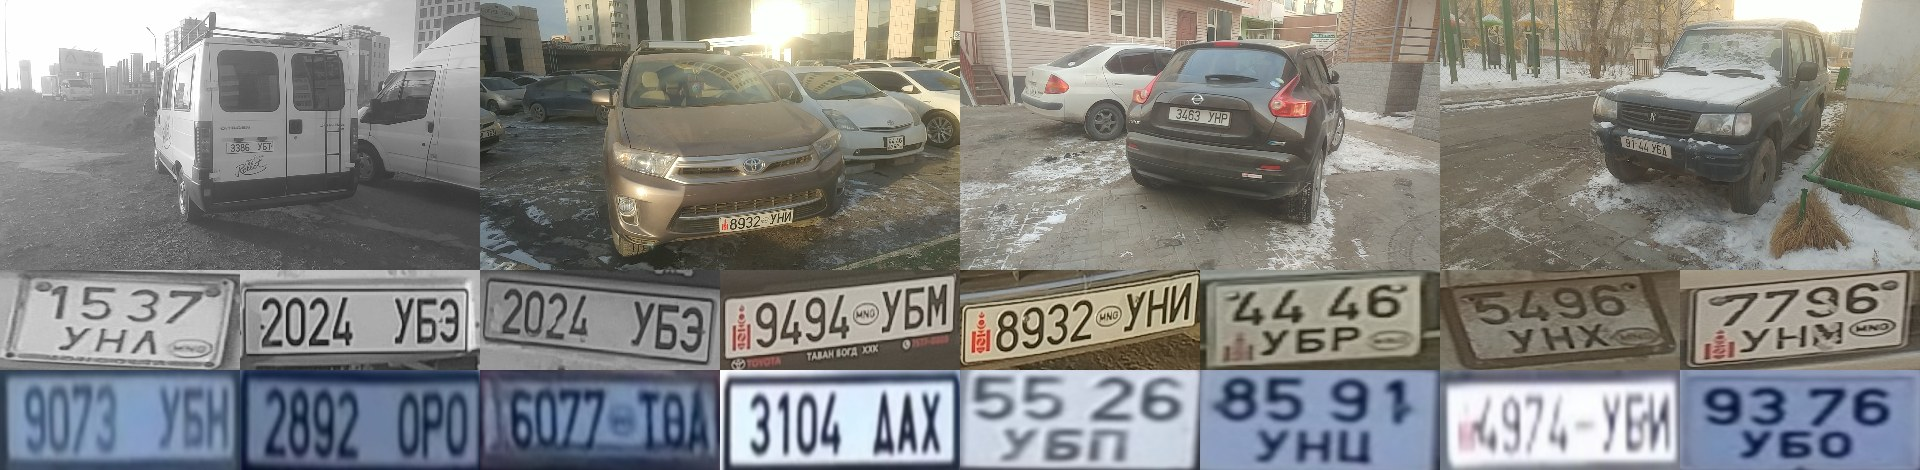
\includegraphics[width=\textwidth]{samples_real.jpg}
\caption{Бодит өгөгдлийн жишээ. Дээд мөр: gumbernator/Mongolian-ALPR олонлогийн бүтэн дүрстэй зураг (Улаанбаатар, зогсоол, өвлийн өдөр, гар утас, 1920$\times$1080). Дунд мөр: тэдгээрийн дугаарын тайралт --- нэг мөрт, зураастай хуучин, хоёр мөрт хэлбэрүүд. Доод мөр: MLUB тэмцээний замын камерын тайралт (470$\times$110, хоёр мөрт дугаар сунгагдсан).}\label{fig:samples}\end{figure}

\section{Өгөгдлийн эх үүсвэрүүд}
Нээлттэй эх үүсвэрийг GitHub, Roboflow Universe, HuggingFace, Kaggle дээр хайж, олдсон бүх зүйлийг Хүснэгт~\ref{tab:sources}-д нэгтгэв. Хэмжээг Зураг~\ref{fig:dataset}-д харуулав.
\begin{table}[H]\centering\caption{Судалсан өгөгдлийн эх үүсвэрүүд ба тэдгээрийн ашиглалт}\label{tab:sources}\footnotesize
\begin{tabular}{p{4.2cm}p{2.2cm}p{3cm}p{5.2cm}}\toprule
Эх үүсвэр & Хэмжээ & Шошго & Ашиглалт\\\midrule
gumbernator/Mongolian-ALPR (GitHub, Apache-2.0)~\cite{gumbernator} & 68 зураг 1920$\times$1080, 74 дугаар & Pascal VOC: дугаарын хайрцаг + тэмдэгт бүрийн хайрцаг (латин галиг) & тэмдэгтийн хайрцгаас 72 дугаарын текст сэргээсэн; илрүүлэгчийн тохируулга (48), уншигчийн тохируулга (74 мөр), төгсгөл хүртэлх тест (18 зураг, 19 дугаар)\\
MLUB ``Mongolian car plate prediction'' (Tsundgerhen репо дотор)~\cite{tsund} & 7\,394 тайралт 470$\times$110, 5\,575 ялгаатай дугаар & \texttt{training.csv}, \texttt{test.csv}: дугаарын текст & дүрэмд нийцэхгүй 2-ыг хасч 7\,392; уншигчийн гол сургалт (5\,901) ба тест (1\,491)\\
keremberke/license-plate-object-detection (HuggingFace) & 8\,823 зураг (6\,176/1\,765/882) & COCO хайрцаг, 1 анги & илрүүлэгчийн урьдчилсан сургалт (A үе), тест\\
Roboflow Universe computer-vision-m1xzb/mongolian-plate~\cite{roboflowmn} & 984 зураг, 2 хувилбар (2025-04-13) & зөвхөн хайрцаг, CC BY 4.0 & татахад бүртгэл, API түлхүүр шаардлагатай тул татаагүй; \texttt{scripts/download\_roboflow.py} бэлэн\\
Синтетик үүсгэгч (энэ ажил) & 60\,000 дугаар $\to$ 90\,021 мөр & текст & уншигчийн урьдчилсан сургалт\\
Tsundgerhen репогийн бичлэг & 3 бичлэг, 30 fps & шошгогүй & олон кадрын чанарын туршилт\\
Kaggle mlub-mongolian-car-plate-prediction-v1 & 34 KB CSV & текст, зураггүй & ашиглаагүй\\\bottomrule
\end{tabular}\end{table}
\begin{figure}[H]\centering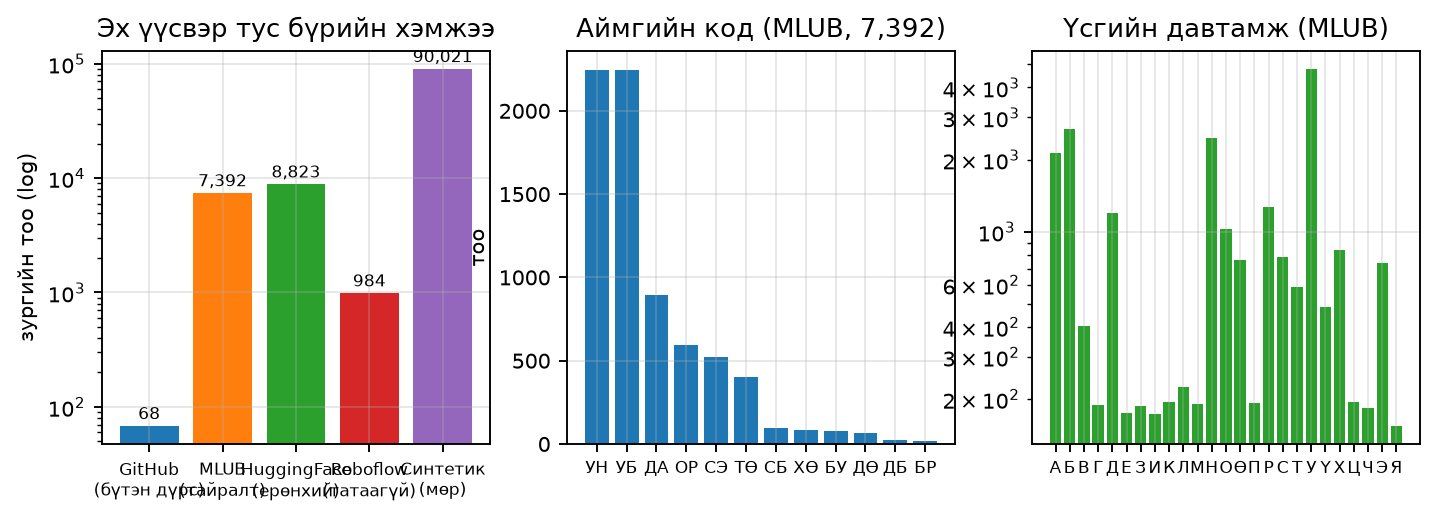
\includegraphics[width=\textwidth]{dataset_overview.png}
\caption{Өгөгдлийн тойм: эх үүсвэр тус бүрийн хэмжээ (зүүн, логарифм), MLUB дугаарын аймгийн кодын тархалт (дунд), MLUB дугаарын үсгийн давтамж (баруун, логарифм). Аймгийн кодоос болж У, Б, Н, А үсэг давамгайлж, серийн үсгүүд ховор байна.}\label{fig:dataset}\end{figure}

\section{Тэмдэгтийн хайрцгаас текст сэргээх}
gumbernator олонлогийн XML файлд дугаарын хайрцаг ба тэмдэгт бүрийн хайрцаг латин галигаар (\texttt{uu}=Ү, \texttt{q}=Ө, \texttt{ye}=Е, \texttt{e}=Э, \texttt{ts}=Ц, \texttt{ch}=Ч, \texttt{ya}=Я гэх мэт) шошголсон байв. Галигийг тэмдэгт бүрийн тайралтыг нүдээр шалгаж баталгаажуулсан. Дугаар тус бүрт түүний дотор орших тэмдэгтийн хайрцгуудыг тоо ба үсэг гэж салгаж, $x$ координатаар эрэмбэлж залгахад дугаарын текст гарна; 4 орон + 3 үсэг бүрдээгүй 2 дугаарыг хаяж 72 дугаар авав. Хоёр мөрт дугаарын хувьд тооны хайрцгуудын нэгдэл ба үсгийн хайрцгуудын нэгдлийг тус тусад нь мөрийн тайралт болгож (\plate{1537} ба \plate{УНЛ}), нэг мөрт дугаарыг бүтнээр нь нэг мөр болгов. Дугаарын хайрцгийн өргөн/өндрийн харьцаа хоёр хэлбэрийг цэвэр ялгаж байгааг Зураг~\ref{fig:aspect}-д харуулав: хоёр мөрт 0.98--1.53, нэг мөрт 1.89--3.81, босго 1.8.
\begin{figure}[H]\centering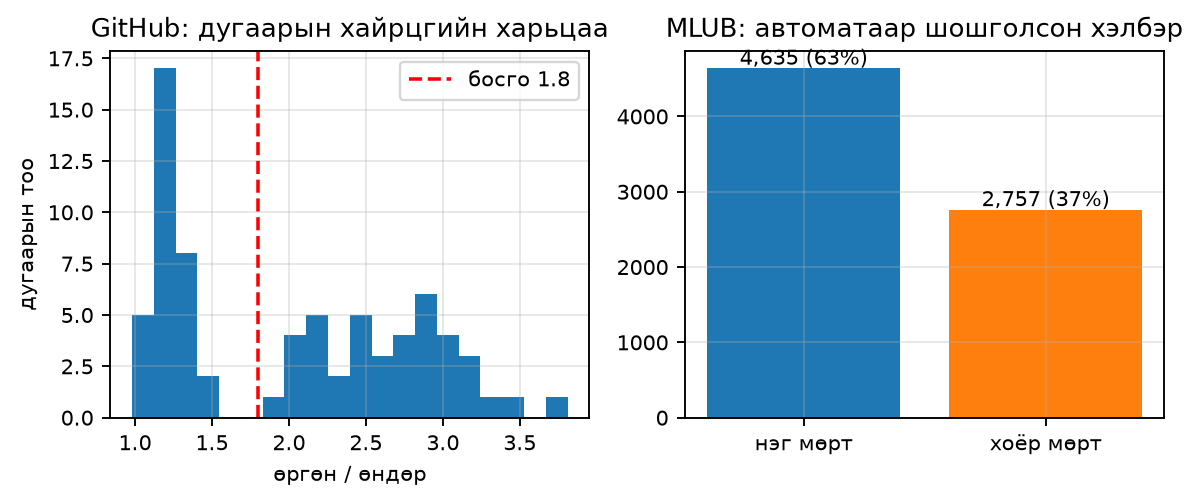
\includegraphics[width=0.95\textwidth]{aspect_layout.png}
\caption{Зүүн: GitHub олонлогийн дугаарын хайрцгийн өргөн/өндөр харьцааны гистограм ба 1.8 босго. Баруун: MLUB тайралтын автоматаар шошголсон хэлбэр (2\,757 буюу 37 хувь нь хоёр мөрт).}\label{fig:aspect}\end{figure}

\section{MLUB тайралтын хэлбэрийг автоматаар шошголох}
MLUB-ийн бүх зураг 470$\times$110 болгож сунгасан тул хоёр мөрт дугаарын хэлбэрийг харьцаагаар ялгах боломжгүй, хэлбэрийн шошго ч байхгүй. Уншигч нэг мөрийг л уншдаг тул сургалтын өмнө хэлбэрийг тодорхойлох шаардлагатай. Үүнд одоо байгаа уншигчийг ашиглан дараах дүрмийг хэрэглэв: (а) зургийг бүтнээр нь уншина; (б) дээд 55 хувь ба доод 55 хувийг тусад нь уншиж залгана; (б) үнэн текстийг яг гаргавал хоёр мөрт, үгүй бол (а) гаргавал нэг мөрт; аль нь ч биш бол засварлах зайгаар (edit distance) ойр нь; тэнцвэл хэвтээ бэхний профилийн тест. Хоёр хагасыг тусад нь уншихад тоо ба үсэг яг гарах нь зөвхөн хоёр мөртэй зурагт боломжтой тул хуваасан тестийг давуу эрхтэй болгосон. Анхны хувилбарт зайн зөрүүг 2-оос багагүй шаардсан нь хоёр мөртийг 571 гэж дутуу шошголсон; дүрмийг засч дахин ажиллуулахад 2\,757 хоёр мөрт (37 хувь), тэнцсэн 87 тохиолдол гарсан. Нэг мөрт гэж шошголсон 36 санамсаргүй зургийг нүдээр шалгахад 1 нь хоёр мөрт байсан тул шошгоны алдаа 3 хувь орчим гэж үзэв.

\section{Сургалт, шалгалтын хуваалт}
Бүх хуваалтыг \emph{дугаарын текстээр} хийв: нэг машин хэд хэдэн зурагт байвал бүгд нэг талд орно (Зураг~\ref{fig:splits}). GitHub олонлогийг 70/30 хуваахад 48 сургалт / 18 шалгалтын зураг (53 / 19 дугаар, 74 / 30 мөр), давхцал тэг. MLUB-ийн тэмцээний анхны training/test хуваалтыг ашиглах боломжгүй, учир нь тестийн зураг нь сургалтын машинуудын нэмэлт кадрууд (3\,150 дугаар давхцсан); иймд 5\,575 ялгаатай дугаарыг 80/20 хуваахад 5\,901 сургалт / 1\,491 тестийн тайралт (8\,094 / 2\,055 мөр), давхцал тэг. HuggingFace олонлогийн анхны 6\,176/1\,765/882 хуваалтыг хэвээр ашиглав. GitHub олонлог нь камер, зургийн хүрээ (бүтэн машин, гар утас) өөр тул илрүүлэгч + уншигчийн төгсгөл хүртэлх тестийн үүрэг гүйцэтгэнэ.
\begin{figure}[H]\centering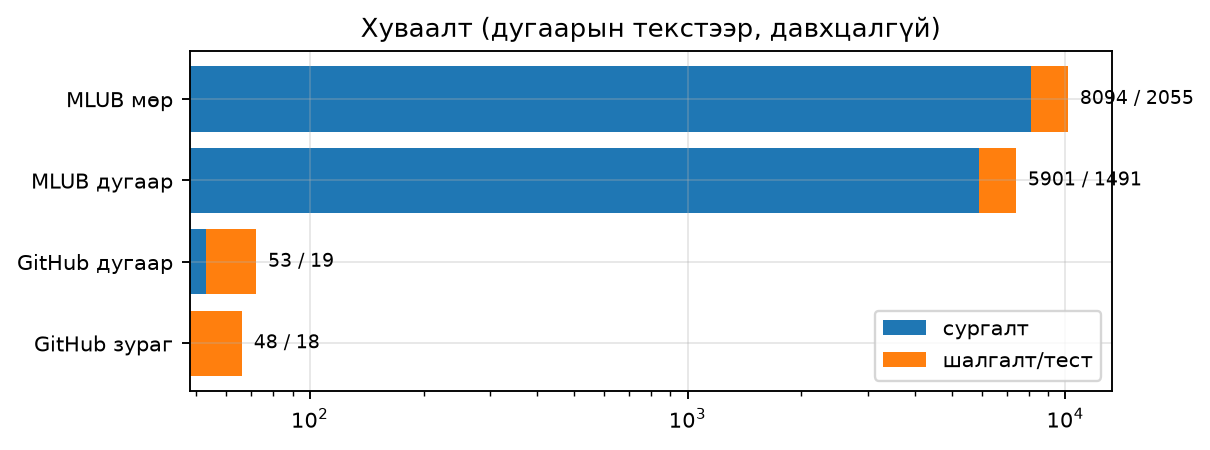
\includegraphics[width=0.85\textwidth]{splits.png}
\caption{Хуваалтын хэмжээ (логарифм тэнхлэг). Бүх хуваалт дугаарын текстээр хийгдсэн тул нэг дугаар сургалт, шалгалтын аль алинд байхгүй.}\label{fig:splits}\end{figure}

\section{Синтетик дугаар үүсгэх}
Уншигч 45 тэмдэгтийн ангийг 74 бодит мөрөөс сурах боломжгүй тул монгол дугаарын дизайныг дуурайсан синтетик үүсгэгч бичив (\texttt{scripts/synth\_plates.py}, Зураг~\ref{fig:synth}). Нэг дээж үүсэх алхмууд:
\begin{enumerate}[leftmargin=2.5em]
\item \textbf{Текст.} Дөрвөн орон санамсаргүй; аймгийн код 29 кодоос ажиглагдсан давтамжаар жинлэж (УБ 40, УН 25, УА 6, УЕ 4, УК 3 хувь, бусад тус бүр 1.2 хувь орчим), 10 хувьд бүрэн санамсаргүй хоёр үсэг (35 үсэг бүгд сургалтад орох үүднээс); серийн үсэг дугаар дээр ажиглагдсан 25 үсгээс 90 хувь, бүх үсгээс 10 хувь.
\item \textbf{Зурах.} PIL сангаар цагаан дэвсгэр (RGB 225--255), хар хүрээ (3--10~px), бэх (0--30). Нэг мөрт 1040$\times$220~px (50 хувь): Соёмбо + тоо + MNG зууван + үсэг (55 хувь), зураастай хуучин хэлбэр (25 хувь), энгийн (20 хувь). Хоёр мөрт 300--360$\times$220--280~px (50 хувь): дээд мөр Соёмбо + тоо, доод мөр үсэг; үүнээс дээд ба доод мөрийн хоёр тайралт гаргана. Соёмбог яг хуулбарлах фонт байхгүй тул улаан гал, нар, сар, зураасны баганаар ойролцоо зурсан. Есөн кирилл фонт (Roboto, Roboto Flex, Roboto Mono, PT Sans Bold, Fira Sans Condensed Medium/SemiBold, Oswald, DejaVu Sans Bold/Condensed Bold, Noto Sans Condensed/SemiCondensed Bold); хувьсах фонтод жин $\{500,600,700\}$, өргөн $\{75,87,100\}$ санамсаргүй.
\item \textbf{Аугментаци} (Хүснэгт~\ref{tab:aug}): илрүүлэгчийн хайрцгийн алдааг дуурайсан захын шилжилт, перспектив, эргүүлэлт, нягтрал бууруулалт, гэрлийн өөрчлөлт, сүүдэр, шороо, шуугиан, бүдэг, JPEG шахалт.
\end{enumerate}
60\,000 дугаараас 90\,021 мөр зураг (нэг мөрт 1, хоёр мөрт 2 мөр) үүсгэхэд 5 минут зарцуулав.
\begin{table}[H]\centering\caption{Синтетик дугаарын аугментацийн параметрүүд}\label{tab:aug}\small
\begin{tabular}{llc}\toprule
Хувиргалт & Параметр & Магадлал\\\midrule
Захын шилжилт (тайралтын зах) & өндөр/өргөний $-4\ldots+12$ хувь, дурын өнгөт зах & 1.0\\
Перспектив & булан $\pm8$ хувь өргөн, $\pm12$ хувь өндөр & 0.8\\
Эргүүлэлт & $\pm8^\circ$ & 0.7\\
Нягтрал бууруулах & өндөр $\{14,16,20,24,24,28,32,32,40,48,64\}$~px & 1.0\\
Тод байдал, offset & $\times0.55\ldots1.25$, $\pm35$ & 1.0\\
Өнгөний хазайлт & суваг бүрт $\pm15$ & 1.0\\
Гамма & $0.6\ldots1.6$ & 0.5\\
Сүүдрийн зурвас & санамсаргүй дөрвөлжин, 50 хувь харанхуй & 0.4\\
Шороо, толбо & 1--5 тойрог, радиус 1--4 & 0.3\\
Gaussian шуугиан & $\sigma\in[0,12]$ & 1.0\\
Gaussian бүдэг & цөм 3 эсвэл 5 & 0.5\\
Хөдөлгөөний бүдэг & цөм 3, 5, 7 (хэвтээ) & 0.3\\
JPEG дахин шахалт & чанар 30--90 & 0.6\\
Хар цагаан & & 0.15\\\bottomrule
\end{tabular}\end{table}
\begin{figure}[H]\centering
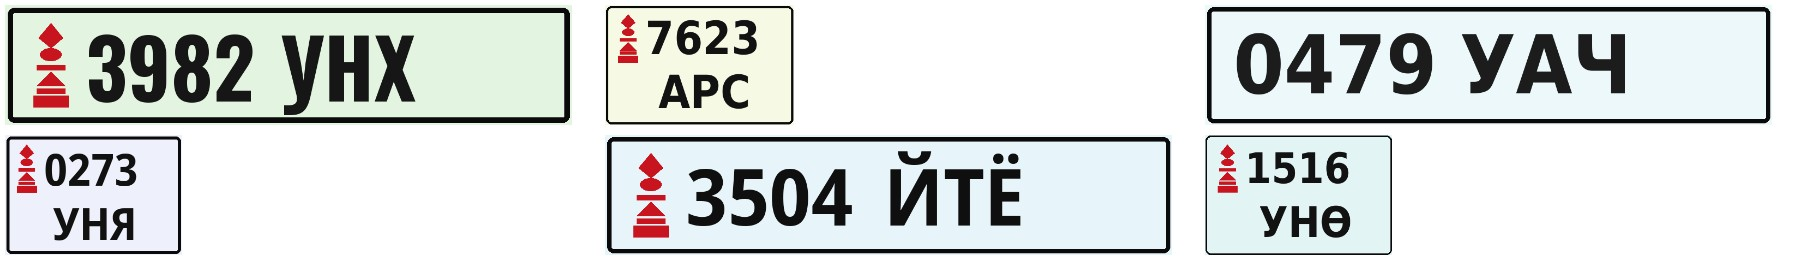
\includegraphics[width=\textwidth]{samples_synth_clean.jpg}\\[2pt]
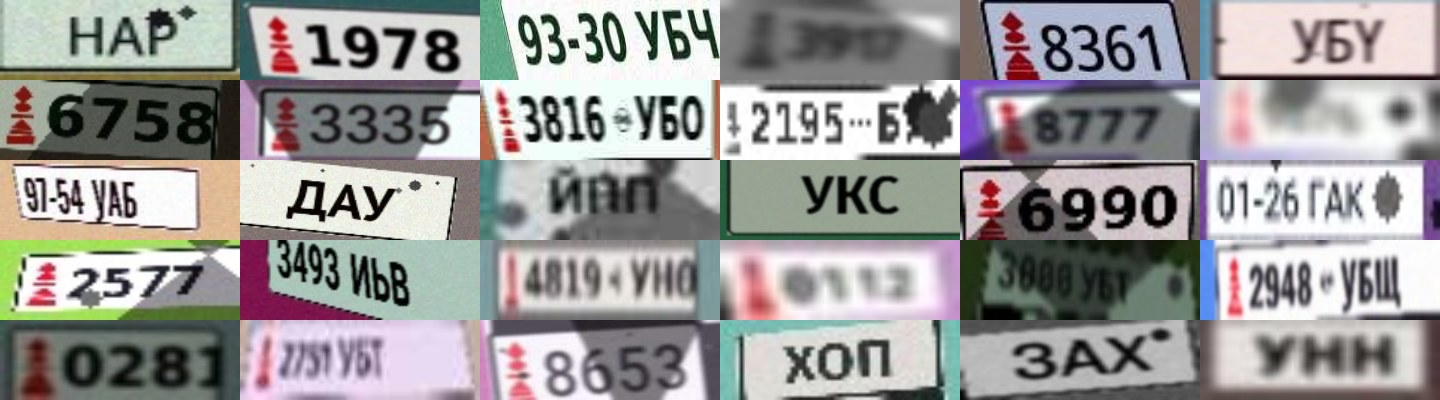
\includegraphics[width=\textwidth]{samples_synth.jpg}
\caption{Синтетик дугаар. Дээд: аугментацийн өмнөх цэвэр рендер (нэг ба хоёр мөрт, Соёмбо, MNG зууван, өөр фонтууд). Доод: аугментацийн дараах сургалтын мөр зургууд (нэг мөрт бүтэн дугаар, хоёр мөрт дугаарын тооны мөр ба үсгийн мөр).}\label{fig:synth}\end{figure}

\section{Шошгоны чанар ба хязгаарлалт}
GitHub олонлогийн тэмдэгтийн шошгыг нүдээр шалгахад галигийн андуурал олдоогүй; тэмдэгт дутуу 2 дугаарыг хассан. MLUB-ийн текст нь тэмцээний зохион байгуулагчийн шошго бөгөөд дүрэмд нийцэхгүй 2 бичлэг (\plate{80213МР}, \plate{0999ТЧ}) олдсон нь шошгоны чанар өндөр гэдгийг илтгэнэ; харин хэлбэрийн шошго автомат тул 3 хувь орчим алдаатай, энэ нь сургалтад хэдэн буруу мөр оруулж, тестэд алдаа гэж тоологдоно. Бодит зураг бүгд өдрийн гэрэлд авсан; шөнө, бороо, гэрлийн гялбааг зөвхөн аугментаци дуурайж байгаа нь энэ өгөгдлийн гол хязгаарлалт юм.

\chapter{ТАНИХ СИСТЕМИЙН АРГА ЗҮЙ}
\section{Системийн ерөнхий бүтэц}
Систем нь Зураг~\ref{fig:pipeline}-д үзүүлсэн таван алхамтай: (1) YOLO11n илрүүлэгч кадраас дугаарын хайрцгийг олно; (2) хайрцгийн өргөн/өндөр харьцаагаар нэг эсвэл хоёр мөрт гэж ангилж, хоёр мөртийг дээд ба доод мөр болгон хуваана; (3) CRNN+CTC уншигч мөр бүрийг текст болгоно; (4) дугаарын дүрэм текстийг нормчилж, хүчинтэй эсэх ба магадлалын оноог тооцно; (5) бичлэгийн хувьд IoU мөрдөлт ба итгэлээр жинлэсэн тэмдэгт тус бүрийн саналаар мөр бүрийн санал нэгдсэн дугаарыг гаргана. Хэрэгжүүлэлт \texttt{mn\_alpr} багцад байна: \texttt{charset.py}, \texttt{plate\_rules.py}, \texttt{crnn.py}, \texttt{pipeline.py}.
\begin{figure}[H]\centering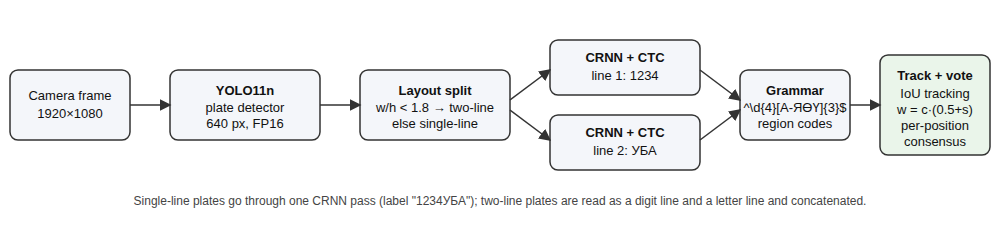
\includegraphics[width=\textwidth]{pipeline.png}
\caption{Системийн боловсруулалтын урсгал. Нэг мөрт дугаар уншигчаар нэг удаа (\plate{1234УБА}), хоёр мөрт дугаар тооны мөр ба үсгийн мөр гэж хоёр удаа орж залгагдана.}\label{fig:pipeline}\end{figure}

\section{Дугаар илрүүлэгч: YOLO11n}
Ultralytics YOLO11n~\cite{yolo11} (2.60 сая параметр, 640~px оролт, 1 анги) загварыг COCO жингээс эхлүүлж хоёр үе шаттай сургав. COCO-ийн 80 ангид дугаар байхгүй тул бэлэн жин дугаар илрүүлэхгүй; иймд \textbf{A үе}: 8\,823 олон улсын зураг дээр 25 эпох --- дугаарын ерөнхий геометрийг сурна; \textbf{B үе}: ерөнхий сургалтын 6\,176 зураг + монгол 48 зураг (hard link-ээр 15 дахин давтаж 720 болгосон) дээр 60 эпох, lr$_0=0.005$ --- монгол дугаарын хайрцгийг нарийн тохируулна. Шалгалт (загвар сонголт) монгол 18 зураг дээр mAP$_{50\text{--}95}$-аар. Нийтлэг тохиргоог Хүснэгт~\ref{tab:dethp}-д үзүүлэв; хэвтээ тусгалыг унтраасан, учир нь дугаарын үсэг толин тусгал болж буруу жишээ үүсгэнэ.
\begin{table}[H]\centering\caption{YOLO11n илрүүлэгчийн сургалтын тохиргоо}\label{tab:dethp}\small
\resizebox{\textwidth}{!}{\begin{tabular}{ll}\toprule
Параметр & Утга\\\midrule
Загвар, эхлэл & YOLO11n, COCO урьдчилан сургасан жин\\
Оролт, batch & 640~px, 32\\
Эпох & A үе 25, B үе 60 (хамгийн сайн эпох 53)\\
Сургалтын хурд & A: Ultralytics анхдагч (lr$_0$ 0.01, warmup 3 эпох); B: lr$_0$ 0.005; cosine бууралт\\
Оптимизатор & Ultralytics auto (SGD/AdamW), weight decay $5\cdot10^{-4}$\\
Алдагдлын жин & box 7.5, cls 0.5, dfl 1.5\\
Аугментаци & mosaic (сүүлийн 10 эпохд унтраана), mixup 0.1, degrees 5, shear 3, perspective 0.0005, HSV анхдагч, \textbf{fliplr 0}\\
Монгол зургийн давталт & 15$\times$ (B үе)\\
Загвар сонголт & монгол шалгалтын mAP$_{50\text{--}95}$\\\bottomrule
\end{tabular}}\end{table}

\section{Хэлбэр тодорхойлох ба мөр хуваах}
Илэрсэн хайрцгийг өргөний 3 хувь, өндрийн 6 хувиар тэлж тайрна. Өргөн/өндөр $<1.8$ бол хоёр мөрт гэж үзэж дээд 55 хувь ба доод 55 хувийг (10 хувь давхцалтай) тусад нь уншиж, тоо + үсэг гэж залгана; үгүй бол бүтнээр нь уншина. Босгыг Зураг~\ref{fig:aspect}-ийн тархалтаас сонгосон.

\section{Уншигч: CRNN + CTC}
Уншигчийн архитектур (Хүснэгт~\ref{tab:crnn}) нь Shi нарын CRNN~\cite{shi2017crnn} ба PaddleOCR-ийн уншигчийн зарчмыг дагасан: residual CNN суурь, хоёр давхар BiLSTM хүзүү, CTC толгой. Оролт: BGR мөр зургийг өндөр 48~px болгож, харьцаа хадгалан өргөнийг 192~px-ээс ихгүй болгоод баруун талд саарал (127) дүүргэж, $[-1,1]$ мужид нормчилно. Тэмдэгтийн олонлог: 10 орон + монгол кирилл 35 үсэг (\texttt{АБВГДЕЁЖЗИЙКЛМНОӨПРСТУҮФХЦЧШЩЪЫЬЭЮЯ}) + CTC blank = 46 анги. Бүх 35 үсгийг оруулсан нь ховор серийн үсгийг дүрслэх боломж олгох бөгөөд аймгийн кодын магадлалыг дүрмийн шат хариуцна. Декод greedy: алхам бүрт хамгийн их магадлалтай анги, давталтыг нэгтгэж blank-ийг хасна; мөрийн итгэл = гаргасан тэмдэгтүүдийн магадлалын дундаж.
\begin{table}[H]\centering\caption{CRNN уншигчийн архитектур (оролт $3\times48\times192$, нийт 9.45 сая параметр)}\label{tab:crnn}\small
\resizebox{\textwidth}{!}{\begin{tabular}{llll}\toprule
Давхарга & Тохиргоо & Гаралт ($C\times H\times W$) & Тайлбар\\\midrule
Stem & Conv3$\times$3 + BN + ReLU & $32\times48\times192$ & \\
ResBlock 1 & 32$\to$64, stride (2,2) & $64\times24\times96$ & BasicBlock: 2$\times$Conv3$\times$3+BN, 1$\times$1 shortcut\\
ResBlock 2 & 64$\to$128, stride (2,2) & $128\times12\times48$ & \\
ResBlock 3 & 128$\to$128 & $128\times12\times48$ & \\
ResBlock 4 & 128$\to$256, stride (2,1) & $256\times6\times48$ & өргөнийг хадгална\\
ResBlock 5 & 256$\to$256 & $256\times6\times48$ & \\
ResBlock 6 & 256$\to$384, stride (2,1) & $384\times3\times48$ & \\
ResBlock 7 & 384$\to$384 & $384\times3\times48$ & \\
AdaptiveAvgPool & өндөр $\to1$ & $T=48$ алхам $\times384$ & дараалал\\
BiLSTM & 2 давхар, hidden 192/чиглэл, dropout 0.1 & $48\times384$ & \\
Linear & $384\to46$ & $48\times46$ & CTC логит\\\bottomrule
\end{tabular}}\end{table}

\section{Уншигчийн сургалтын тохиргоо ба үе шат}
Сургалтыг Хүснэгт~\ref{tab:rechp}-ийн тохиргоогоор дөрвөн үе шаттай явуулав (Хүснэгт~\ref{tab:stages}): эхлээд зөвхөн синтетик, дараа нь бодит өгөгдлийг шат дараалан нэмж, өмнөх шатны хамгийн сайн жингээс үргэлжлүүлнэ. Бодит мөрүүдийг эпох бүрт давтаж (GitHub 40$\times$, MLUB 3$\times$) синтетиктэй тэнцвэржүүлсэн. Загвар сонголтын оноо: бүтэн дугаарын нарийвчлал хасах CER, шалгалтын олонлог дээр. MLUB-ийн хэлбэрийн шошго уншигчаас хамаардаг тул 3 дугаар үеийг хоёр удаа ажиллуулав: эхний загвараар дахин шошголж, дараа нь дахин сургав.
\begin{table}[H]\centering\caption{CRNN уншигчийн сургалтын тохиргоо, бүх үе шатанд ижил}\label{tab:rechp}\small
\resizebox{\textwidth}{!}{\begin{tabular}{ll}\toprule
Параметр & Утга\\\midrule
Алдагдал & CTC (blank 0, zero\_infinity)\\
Оптимизатор & AdamW, weight decay $10^{-4}$\\
Хуваарь & OneCycleLR, pct\_start 0.1, дээд lr үе шатаар ($10^{-3}$, $3\cdot10^{-4}$, $5\cdot10^{-4}$)\\
Batch, нарийвчлал & 256, bfloat16 autocast\\
Gradient clipping & 5.0\\
Бодит мөрийн аугментаци & захын шилжилт (0.5), эргүүлэлт $\pm6^\circ$, масштаб 0.9--1.1 (0.5), тод байдал $\times0.6$--1.3, offset $\pm30$, шуугиан $\sigma\le8$, бүдэг 3~px (0.3)\\
Загвар сонголт & plate\_acc $-$ CER (шалгалтын олонлог)\\
Seed & 0\\\bottomrule
\end{tabular}}\end{table}
\begin{table}[H]\centering\caption{Уншигчийн сургалтын үе шатууд}\label{tab:stages}\small
\resizebox{\textwidth}{!}{\begin{tabular}{clccl}\toprule
Үе & Сургалтын өгөгдөл (мөр) & Эпох & Дээд lr & Шалгалт (сонголт)\\\midrule
1 & синтетик 90\,021 & 10 & $10^{-3}$ & GitHub 30 мөр\\
2 & синтетик + GitHub 74$\times$40 & 6 & $3\cdot10^{-4}$ & GitHub\\
3а & синтетик + MLUB 6\,995$\times$1 + GitHub 74$\times$40 (анхны хэлбэрийн шошго) & 8 & $5\cdot10^{-4}$ & MLUB 1\,763 мөр\\
3б & синтетик + MLUB 8\,094$\times$3 + GitHub 74$\times$40 (засварласан шошго) & 20 & $5\cdot10^{-4}$ & MLUB 2\,055 мөр\\\bottomrule
\end{tabular}}\end{table}

\section{Дугаарын дүрэм}
Уншсан текстийг том үсэг болгож, латин ижил хэлбэрт үсгийг кирилл рүү хөрвүүлж (A$\to$А, B$\to$В, E$\to$Е, K$\to$К, M$\to$М, H$\to$Н, O$\to$О, P$\to$Р, C$\to$С, T$\to$Т, Y$\to$У, X$\to$Х), тусгаарлагчийг хасаад \texttt{\^{}\textbackslash d\{4\}[А-ЯӨҮ]\{3\}\$} загвартай тулгана. Магадлалын оноо $s(y)\in[0,1]$: дүрэмд нийцвэл 0.6, эхний хоёр үсэг 29 аймгийн кодын хүснэгтэд (Хавсралт~\ref{app:regions}) байвал $+0.3$, серийн үсэг дугаар дээр ажиглагдсан 25 үсгийн нэг бол $+0.1$.

\section{Олон кадрын баталгаажуулалт}
Кадр бүрийн илрүүлэлтийг өмнөх мөрүүдтэй IoU $\ge0.3$-аар холбож, 15 кадр дараалан алга болсон мөрийг дуусгана. Мөр $t$ кадрт $y_t$ текст, $c_t$ итгэл авахад саналын жин
\begin{equation}
w_t = c_t\,\bigl(0.5 + s(y_t)\bigr)
\end{equation}
бөгөөд урт $L$ ба байрлал $i$ бүрт $V_L[i][\mathrm{ch}] \mathrel{+}= w_t$ хуримтлуулна. Санал нэгдсэн урт нь нийт масс хамгийн их урт ($L=7$-д 1.3 дахин давуу), байрлал бүрт хамгийн их саналтай тэмдэгтийг сонгож, \emph{margin} = ялсан тэмдэгтүүдийн саналын хувийн дундаж гэж найдвартай байдлын оноо гаргана. Энэ арга нь~\cite{laroca2018}-ын олонхийн саналыг итгэл ба дүрмийн жингээр өргөтгөсөн; ганц тэмдэгтийн андуурлыг бусад кадр засдаг. Зогсоолын хаалганд санал болгож буй шийдвэрийн дүрэм: мөр $\ge3$ кадртай, санал нэгдсэн дугаар дүрэмд нийцсэн, margin $\ge0.8$ бол нээнэ; үгүй бол оператор/интеркомд шилжүүлнэ.

\section{Үнэлгээний хэмжүүр}
\begin{itemize}[leftmargin=2em]
\item \textbf{Илрүүлэлт:} precision, recall, mAP$_{50}$, mAP$_{50\text{--}95}$ (COCO маяг, Ultralytics val).
\item \textbf{Уншилт:} мөрийн нарийвчлал; CER $=$ засварлах зай / үнэн текстийн урт; \textbf{бүтэн дугаарын нарийвчлал} --- долоон тэмдэгт бүгд зөв (хоёр мөртийг залгаж).
\item \textbf{Төгсгөл хүртэлх:} дугаар IoU $\ge0.5$-аар илэрсэн бөгөөд яг зөв уншигдсан бол зөв.
\item \textbf{Олон кадрын симуляци:} тестийн зургийг $K$ удаа санамсаргүй хувиргаж (эргүүлэлт $\pm3^\circ$, шилжилт $\pm3$ хувь, масштаб 0.9--1.1, тод байдал $\times0.7$--1.3, бүдэг, шуугиан) санал авна; $K\in\{1,3,5,9\}$.
\item \textbf{Хугацаа:} 1920$\times$1080 кадр дээр \texttt{process\_frame} бүхэлд нь (илрүүлэлт, тайралт, уншилт, дүрэм), халаалтын дараа 90 давталт, CUDA synchronize.
\end{itemize}

\section{Хэрэгжүүлэлт}
Код Python 3.12, PyTorch 2.11 (CUDA 12.8), Ultralytics 8.4, OpenCV, NumPy дээр бичигдсэн: \texttt{mn\_alpr/} (загвар, дүрэм, урсгал), \texttt{scripts/} (өгөгдөл бэлтгэх, синтетик, сургалт, үнэлгээ, тайлан), \texttt{app/gradio\_app.py} (зураг/бичлэг оруулах туршилтын интерфэйс). Сургалтыг NVIDIA GeForce RTX 5080 (16~GB) дээр хийсэн: илрүүлэгч 85 эпох 1.5 цаг орчим, уншигч 44 эпох 35 минут орчим. Загварууд ONNX (opset 17) хэлбэрт экспортлогдоно (\texttt{scripts/export\_onnx.py}). GPU байхгүй үед урсгал автоматаар CPU дээр FP32-оор ажиллана.

\chapter{ТУРШИЛТ БА ҮР ДҮН}
Энэ бүлэгт илрүүлэгчийн сургалт, уншигчийн үе шаттай сургалт, тэмдэгтийн андуурлын шинжилгээ, төгсгөл хүртэлх ба олон кадрын үр дүн, хугацааны хэмжилт, бичлэгийн туршилтын үр дүнг үзүүлнэ. Бүх хэмжилт 2026 оны 10 дугаар сарын 14-ний сургалтын жингээр, \texttt{scripts/eval\_pipeline.py} скриптээр хийгдсэн; тоонуудыг \texttt{runs/eval/results.json}-д хадгалсан.

\section{Дугаар илрүүлэгчийн үр дүн}
Зураг~\ref{fig:detcurves}-д хоёр үе шатны сургалтын муруйг үзүүлэв. A үед ерөнхий шалгалтын mAP$_{50}$ эхний эпохоос 0.95-аас дээш гарч 25 эпохын эцэст 0.981 болсон нь дугаарын геометр улс орноос үл хамааран ижил гэдгийг илтгэнэ. B үед монгол зураг нэмэгдсэнээр монгол шалгалтын mAP$_{50\text{--}95}$ 0.69-өөс 0.83 хүртэл өссөн бол mAP$_{50}$ 0.99 орчимд тогтвортой байв: нарийн тохируулга дугаарыг \emph{олох} бус \emph{хайрцгийг нарийн тавих} чадварыг сайжруулсан бөгөөд энэ нь хоёр мөрт дугаарын мөр хуваалтад чухал. Сургалтын алдагдал B үеийн эхэнд (шинэ өгөгдөл) бага зэрэг өсөөд тогтмол буурсан; шалгалтын алдагдал 25 эпохоос хойш хэлбэлзэлтэй ч өсөөгүй тул хэт тохирол ажиглагдсангүй. Хүснэгт~\ref{tab:det}-д сургалт, шалгалт, тестийн олонлог тус бүрийн үр дүнг үзүүлэв; ерөнхий тест (882 зураг) ба шалгалт (1\,765) ойролцоо байгаа нь монгол зургаар тохируулахад ерөнхий чадвар алдагдаагүйг харуулна.
\begin{figure}[H]\centering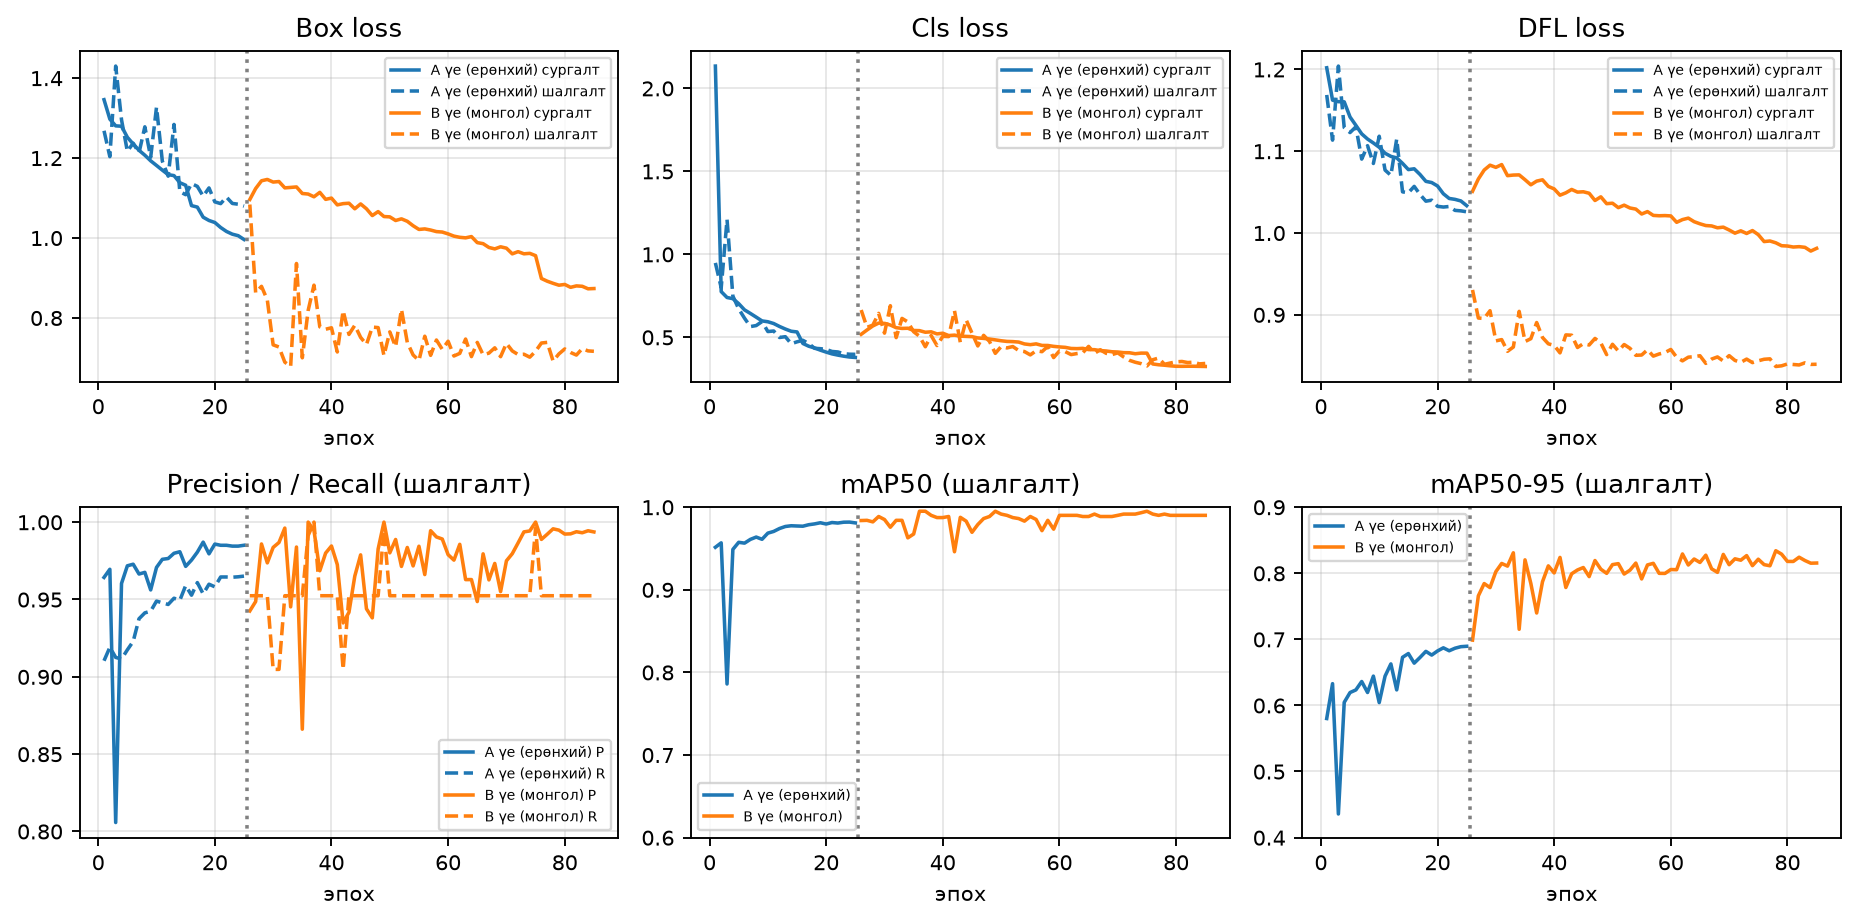
\includegraphics[width=\textwidth]{det_curves.png}
\caption{YOLO11n илрүүлэгчийн сургалтын муруй: box, cls, DFL алдагдал (сургалт --- бүтэн, шалгалт --- тасархай), precision/recall, mAP$_{50}$, mAP$_{50\text{--}95}$ эпох бүрээр. Босоо тасархай шугам A үеэс (ерөнхий 8\,823 зураг) B үе (монгол нэмсэн) рүү шилжсэн цэг; B үеийн шалгалт монгол 18 зураг.}\label{fig:detcurves}\end{figure}
\begin{table}[H]\centering\caption{YOLO11n илрүүлэгчийн үр дүн, 640~px, эцсийн жин (B үеийн 53 дахь эпох)}\label{tab:det}
\resizebox{\textwidth}{!}{\begin{tabular}{lrcccc}\toprule
Олонлог & Зураг & P & R & mAP$_{50}$ & mAP$_{50\text{--}95}$\\\midrule
Монгол шалгалт (GitHub) & 18 (21 дугаар) & 0.996 & 0.952 & \textbf{0.992} & 0.834\\
Ерөнхий шалгалт (HF val) & 1\,765 & 0.974 & 0.970 & 0.982 & 0.699\\
Ерөнхий тест (HF test) & 882 & 0.995 & 0.973 & 0.985 & 0.708\\\bottomrule
\end{tabular}}\end{table}
\begin{figure}[H]\centering
\begin{subfigure}{0.48\textwidth}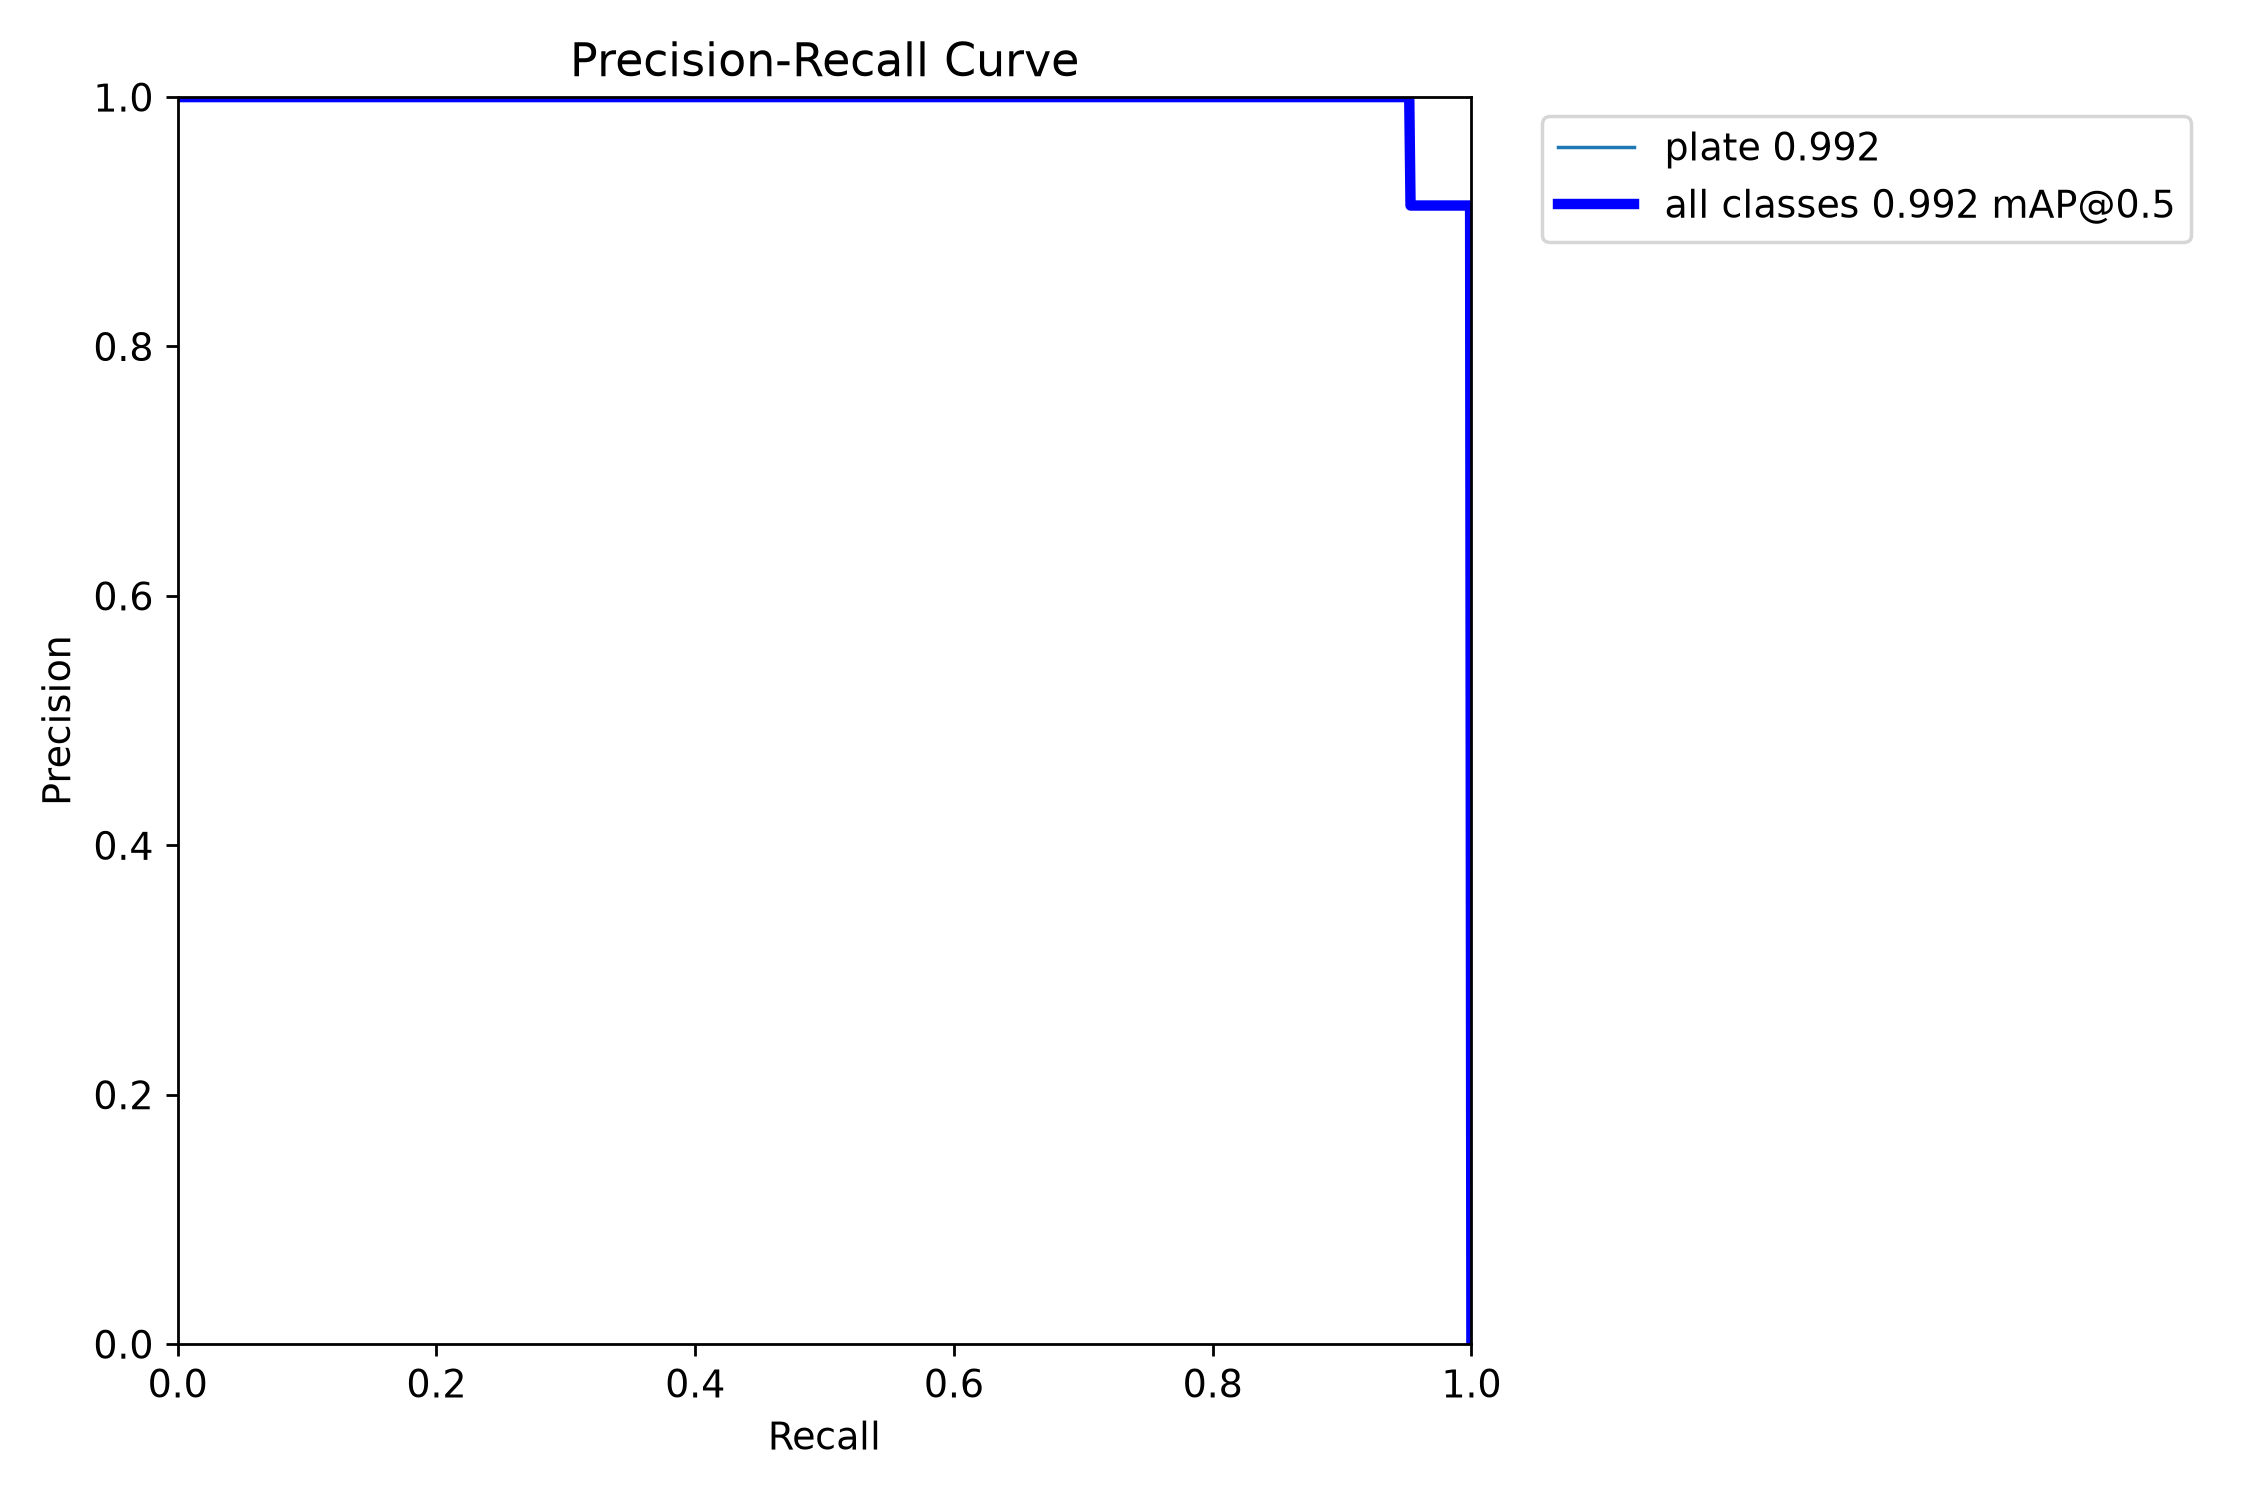
\includegraphics[width=\textwidth]{det_BoxPR_curve.png}\caption{Precision--Recall муруй}\end{subfigure}\hfill
\begin{subfigure}{0.48\textwidth}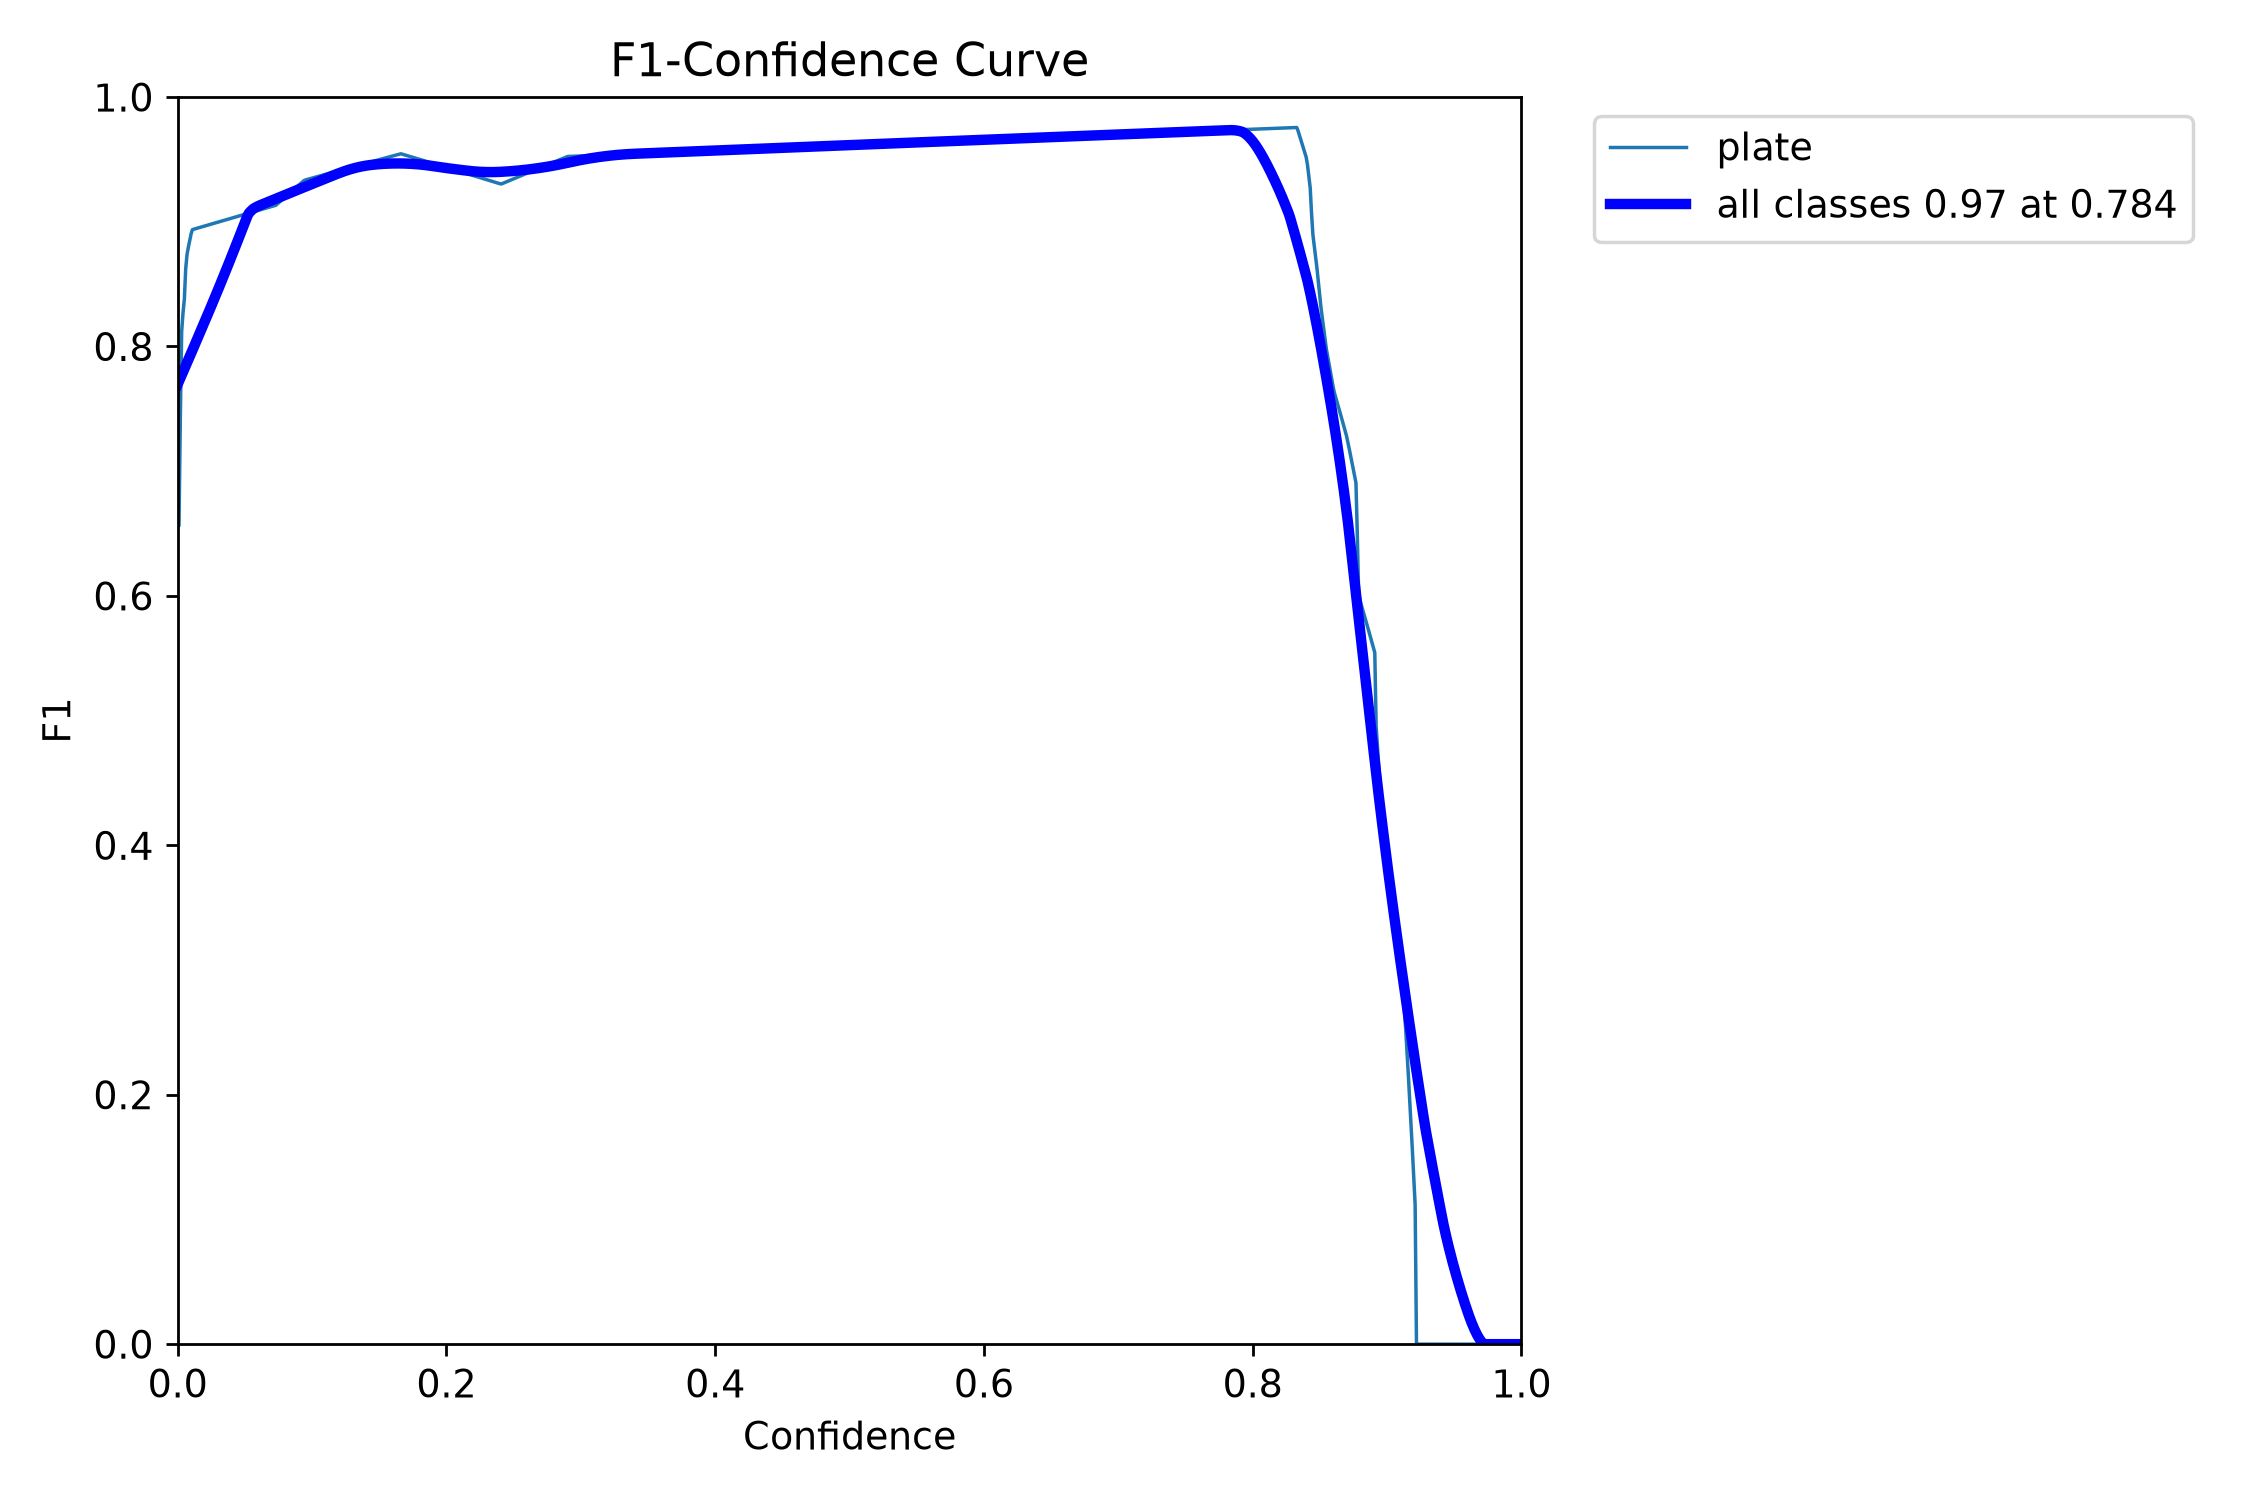
\includegraphics[width=\textwidth]{det_BoxF1_curve.png}\caption{F1--итгэлийн босго муруй}\end{subfigure}
\caption{Илрүүлэгчийн PR ба F1 муруй, монгол шалгалтын олонлог. F1 муруй conf $=0.4$ орчимд хамгийн өндөр байгаа тул урсгалын итгэлийн босгыг 0.4 гэж сонгосон.}\label{fig:detpr}\end{figure}
\begin{figure}[H]\centering
\begin{subfigure}{0.42\textwidth}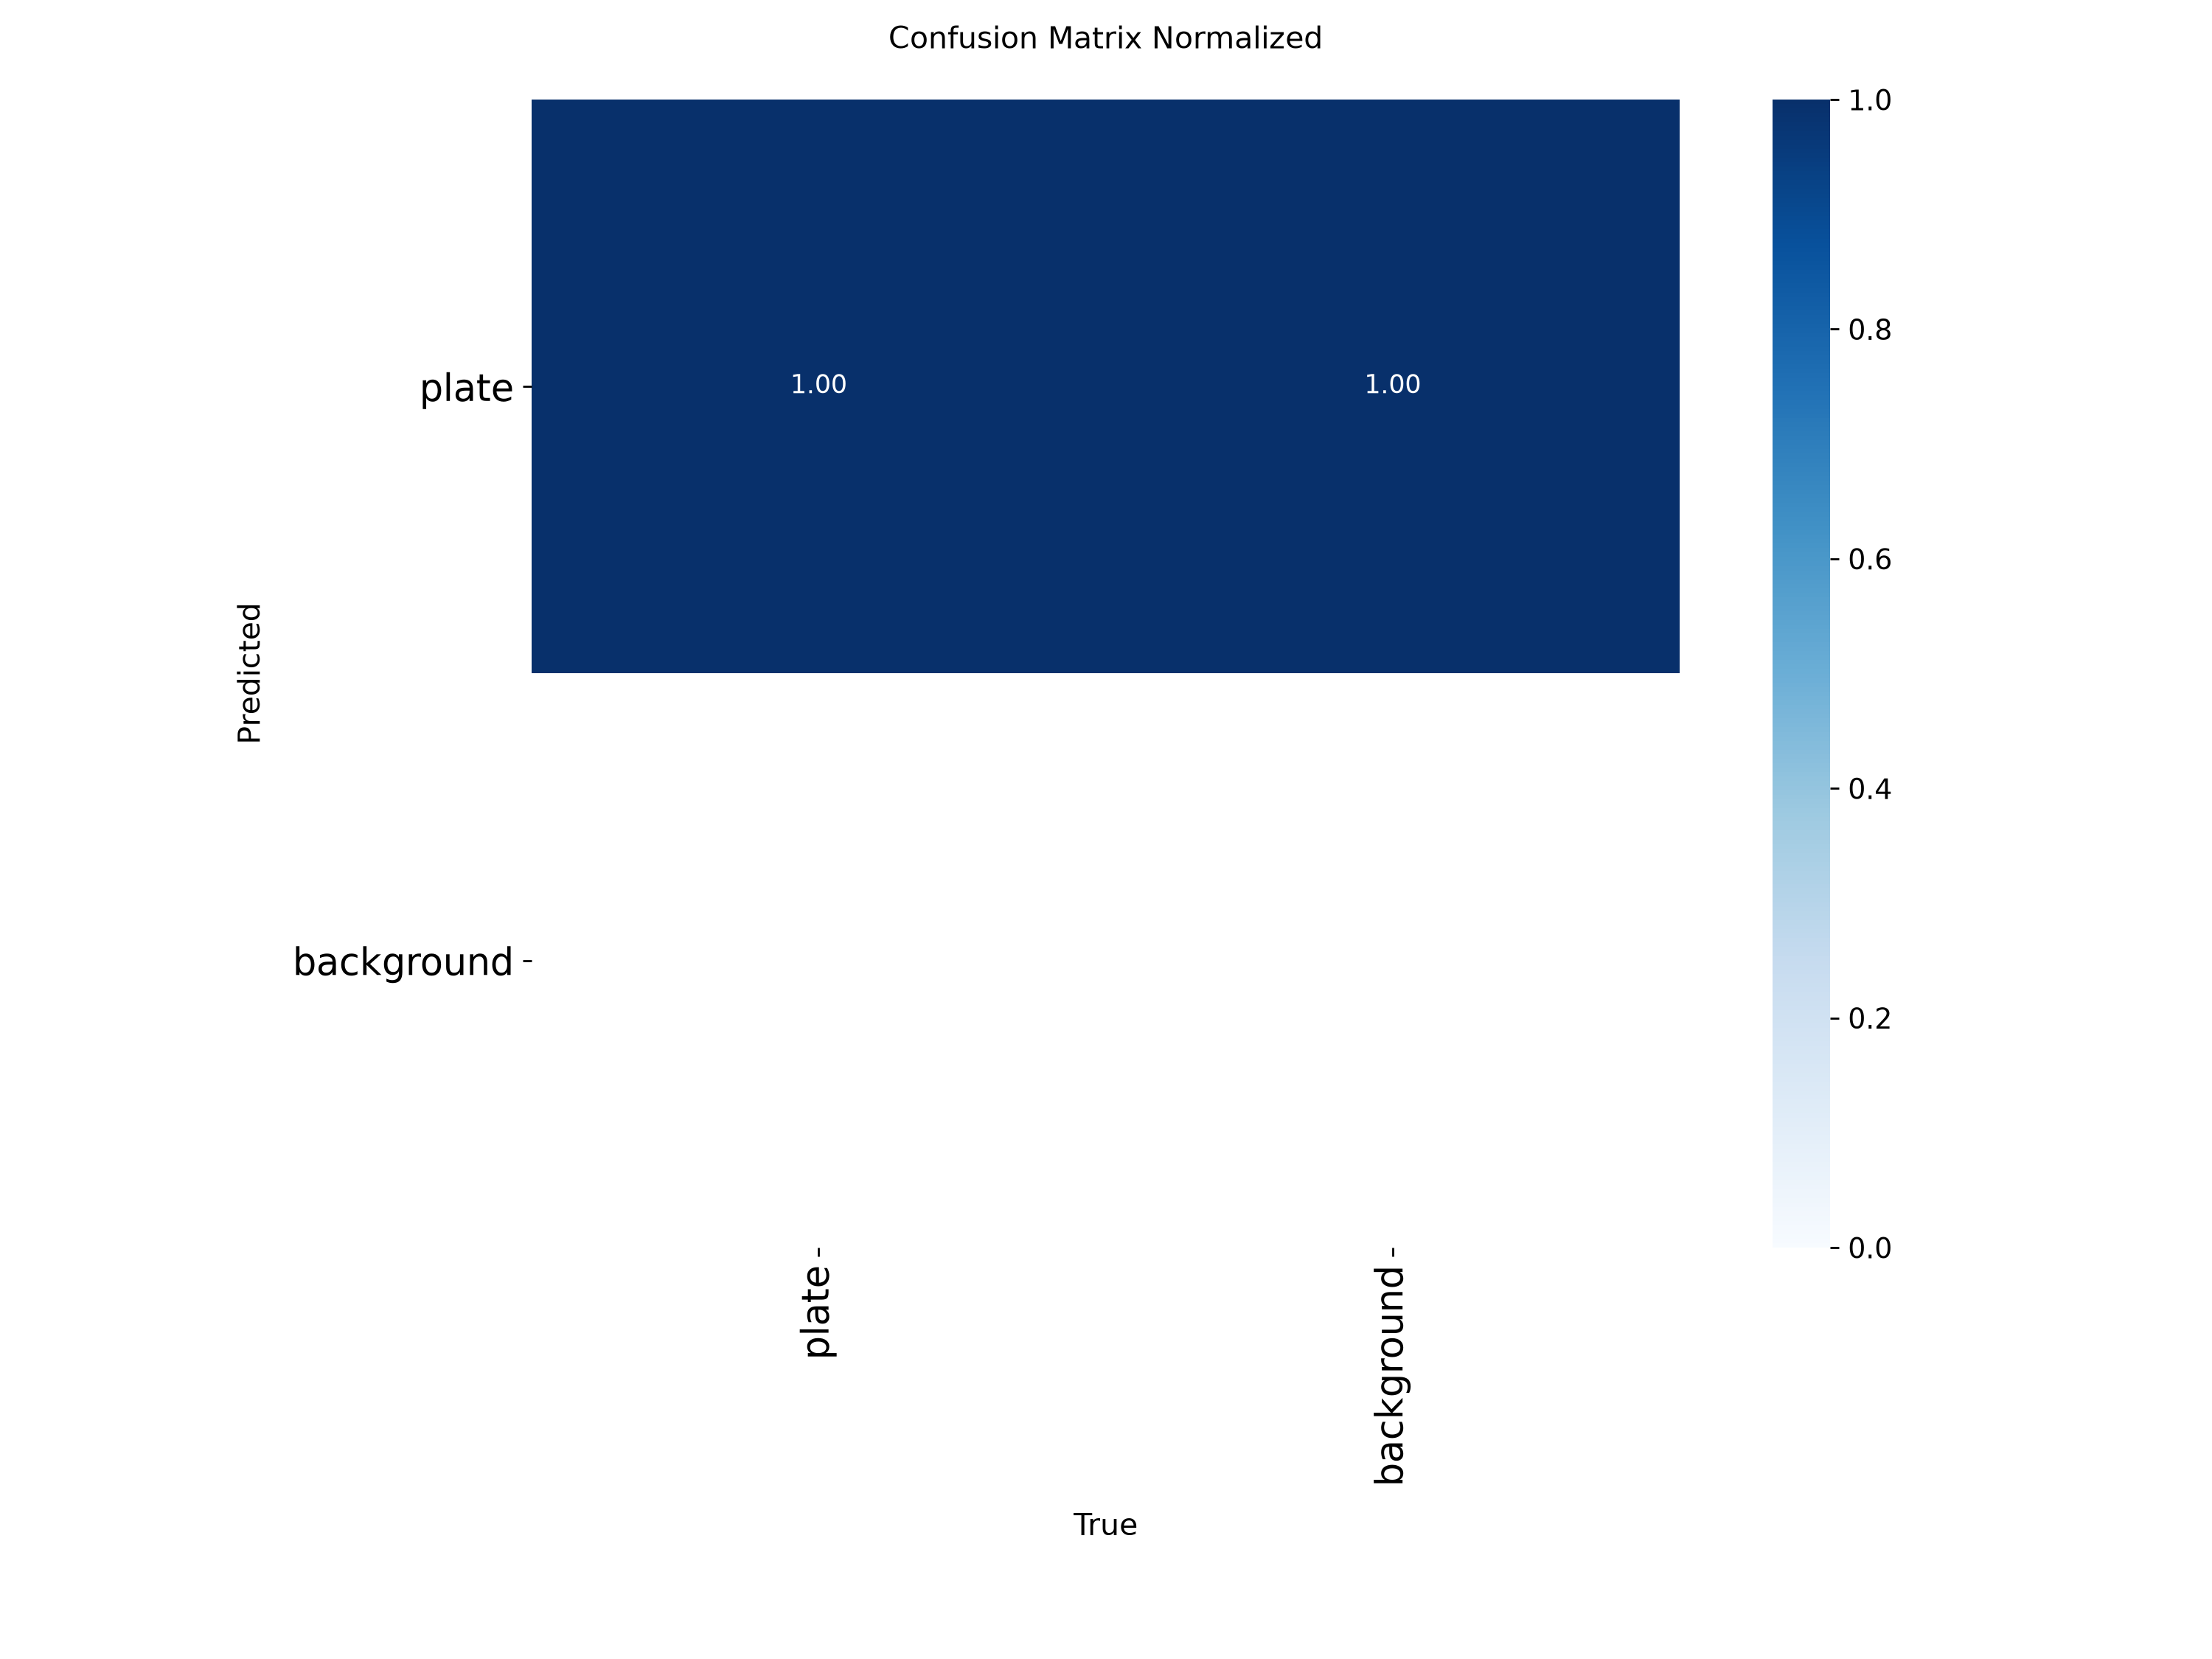
\includegraphics[width=\textwidth]{det_confusion_matrix_normalized.png}\caption{Нормчилсон андуурлын матриц (дугаар / дэвсгэр)}\end{subfigure}\hfill
\begin{subfigure}{0.55\textwidth}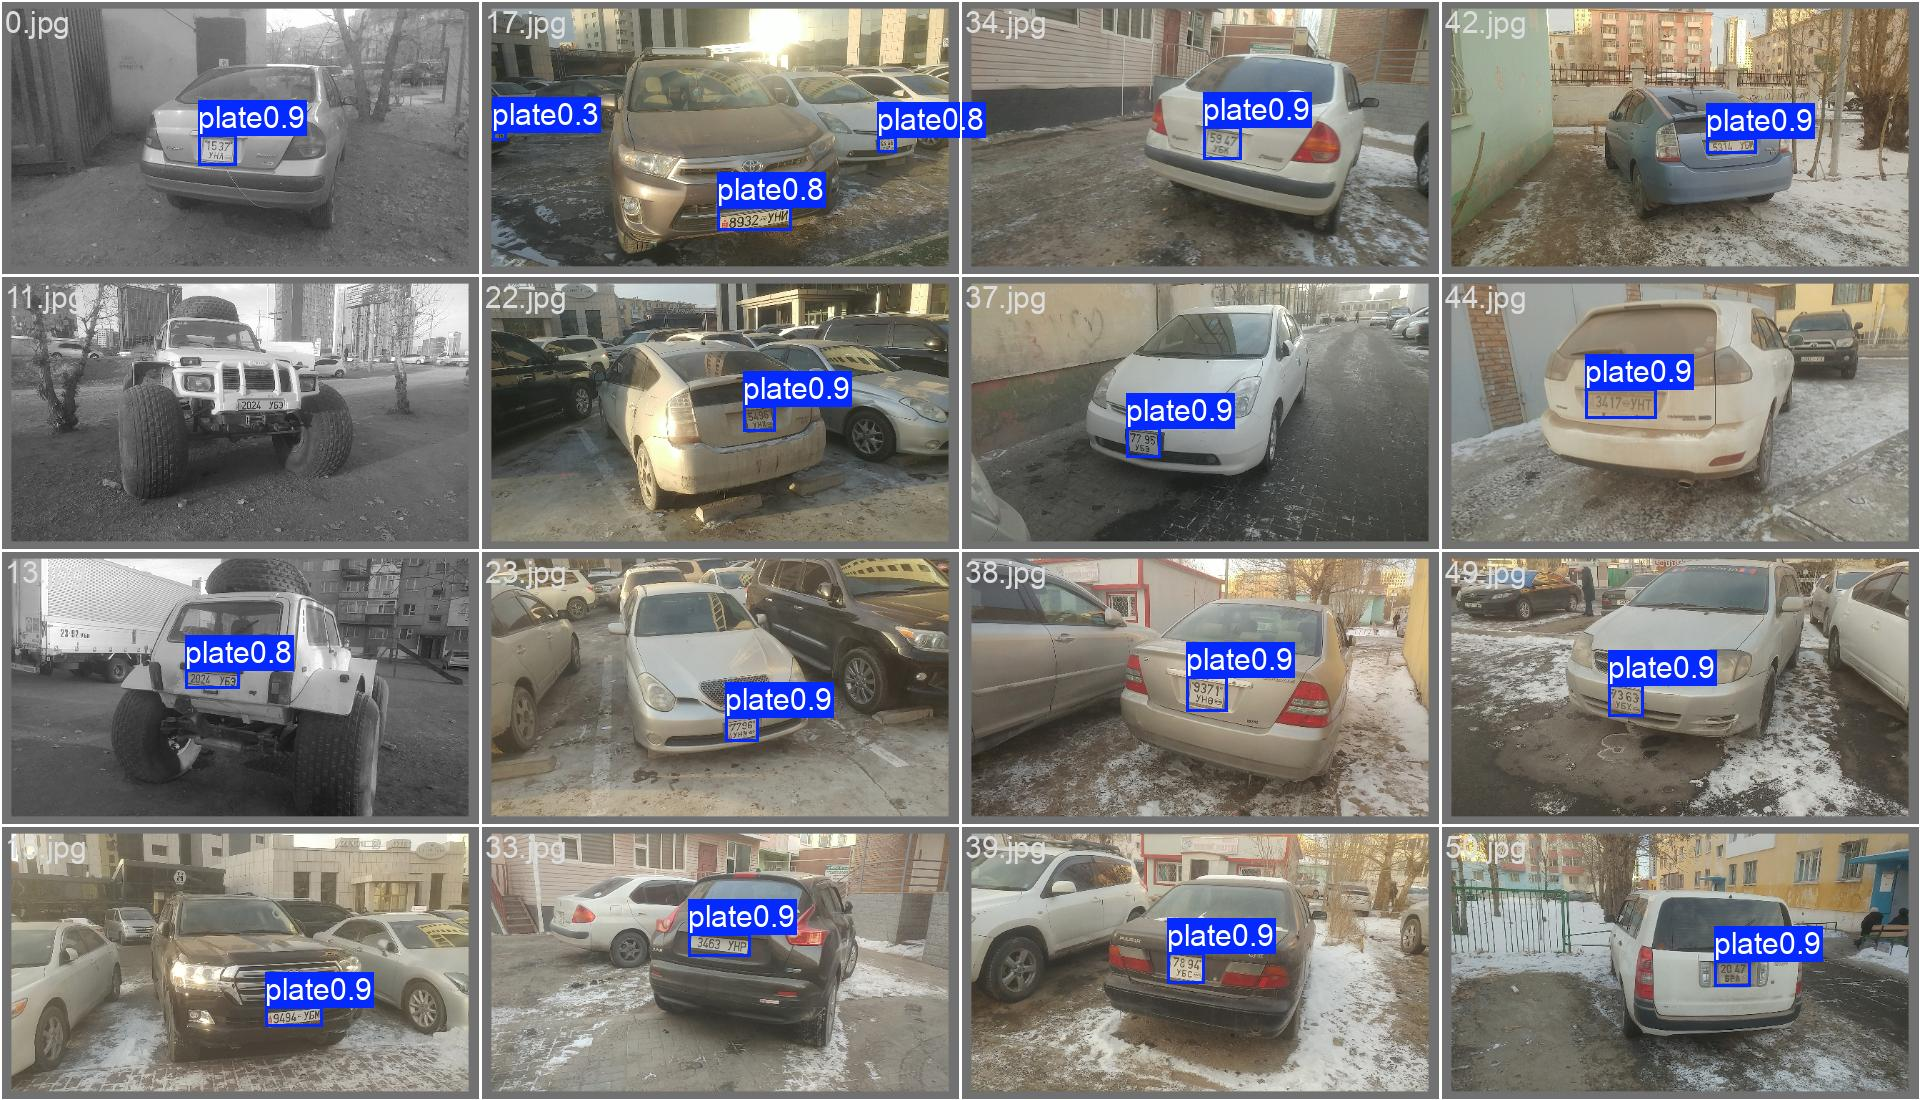
\includegraphics[width=\textwidth]{det_val_batch0_pred.jpg}\caption{Шалгалтын зураг дээрх таамаг}\end{subfigure}
\caption{Илрүүлэгчийн андуурлын матриц ба шалгалтын багцын таамаглал (Ultralytics-ийн гаралт).}\label{fig:detcm}\end{figure}

\section{Уншигчийн сургалтын муруй ба үе шатны нөлөө}
Зураг~\ref{fig:reccurves}-д дөрвөн үе шатны 44 эпохын муруйг үзүүлэв. Зөвхөн синтетикээр (1-р үе) GitHub бодит дугаар дээр 42.1 хувь, CER 0.27 хүрсэн нь рендер дугаарын дизайныг зөв дуурайсан ч бодит камерын шуугиан, бохирдлыг хангалтгүй дуурайж байгааг илтгэнэ. 74 бодит мөр нэмэхэд (2-р үе) эхний эпохдоо 84.2 хувь болж, CER 0.02 хүртэл буурсан --- цөөн ч гэсэн бодит өгөгдөл домэйн зөрүүг ихээхэн хаасан. MLUB нэмсэн 3-р үед шалгалт MLUB-ийн 1\,491 дугаар болж 8 эпохын дараа 91.9 хувь, хэлбэрийн шошгыг засч 20 эпох сургасны дараа 96.8 хувь, CER 0.0064-д хүрсэн. GitHub дугаар дээрх нарийвчлал 3-р үед 84--95 хувийн хооронд хэлбэлзсэн нь 19 дугаарын тест нэг дугаар = 5.3 нэгж хувь гэсэн мөхлөгтэй учир юм. Хүснэгт~\ref{tab:ablation}, Зураг~\ref{fig:ablation}-д үе шат тус бүрийн хамгийн сайн үр дүнг нэгтгэв.
\begin{figure}[H]\centering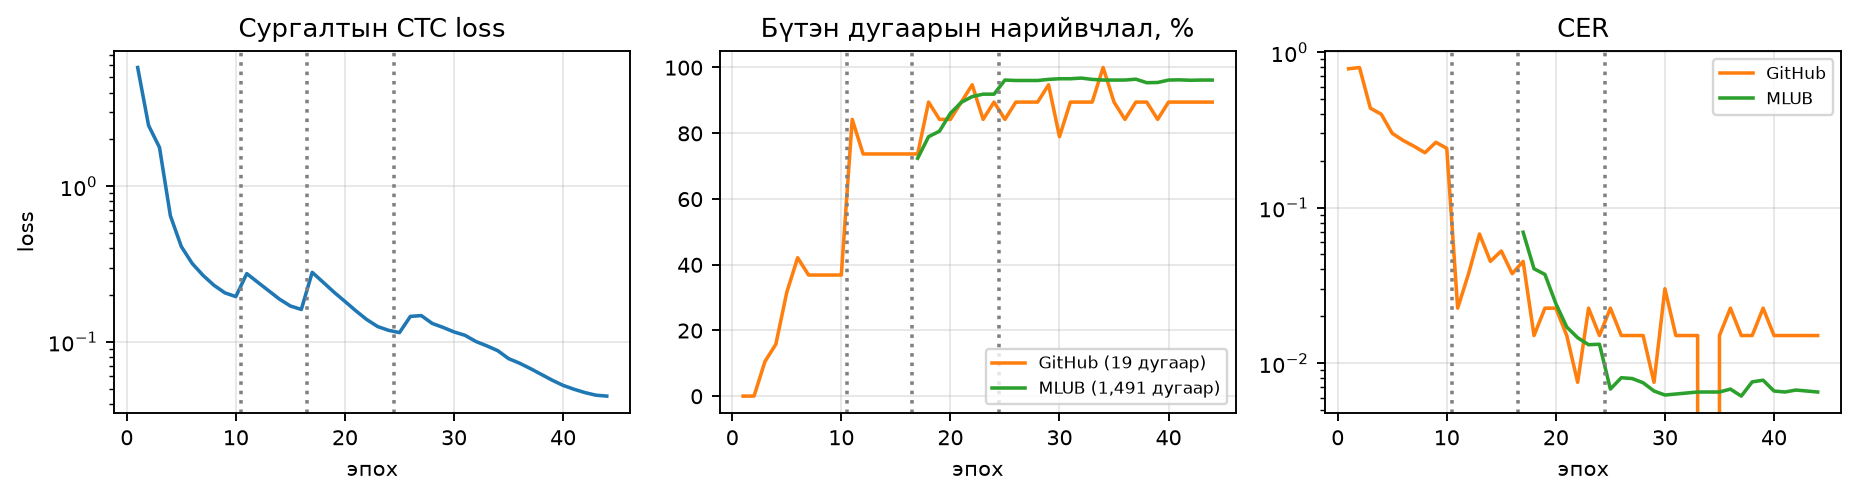
\includegraphics[width=\textwidth]{rec_curves.png}
\caption{CRNN уншигчийн сургалтын муруй, 44 эпох: сургалтын CTC алдагдал (зүүн), бүтэн дугаарын нарийвчлал (дунд), CER (баруун, логарифм). Босоо тасархай шугамууд үе шатны зааг (1: синтетик; 2: +GitHub; 3а: +MLUB; 3б: шошго засч дахин). GitHub муруй 1--2-р үед шалгалт, 3-р үед тест; MLUB муруй 3-р үеийн шалгалт.}\label{fig:reccurves}\end{figure}
\begin{table}[H]\centering\caption{Сургалтын өгөгдлийн нөлөө (ablation): үе шат тус бүрийн хамгийн сайн эпохын үр дүн, бүтэн дугаарын нарийвчлал (хувь) ба CER}\label{tab:ablation}
\resizebox{\textwidth}{!}{\begin{tabular}{lcccc}\toprule
Сургалтын өгөгдөл & GitHub (19), хувь & GitHub CER & MLUB (1\,491), хувь & MLUB CER\\\midrule
Зөвхөн синтетик & 42.1 & 0.271 & --- & ---\\
+ GitHub 74 мөр & 84.2 & 0.023 & --- & ---\\
+ MLUB, анхны шошго (3а) & 84.2 & 0.023 & 91.9 & 0.013\\
+ MLUB, засварласан шошго (3б, эцсийн) & \textbf{89.5} & \textbf{0.015} & \textbf{96.8} & \textbf{0.0064}\\\bottomrule
\end{tabular}}\end{table}
\begin{figure}[H]\centering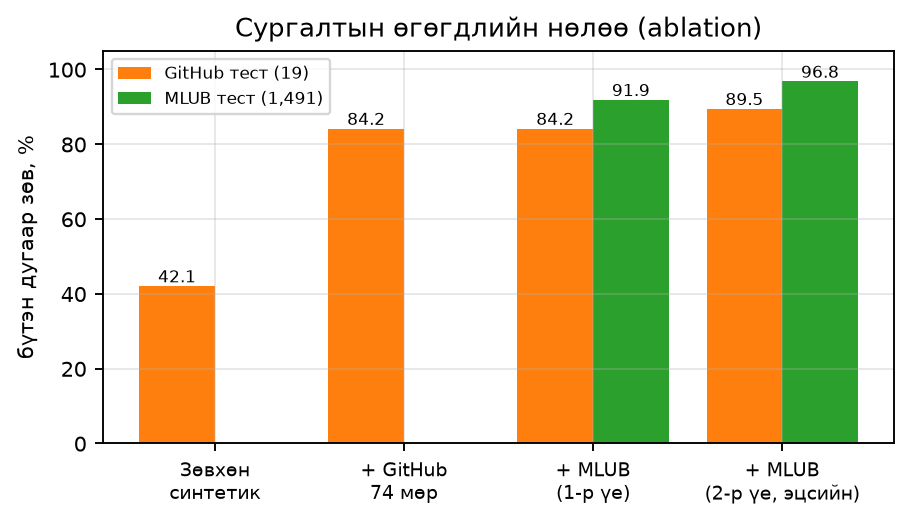
\includegraphics[width=0.7\textwidth]{ablation.png}
\caption{Сургалтын өгөгдлийг шат дараалан нэмэхэд бүтэн дугаарын нарийвчлал хэрхэн өссөн нь.}\label{fig:ablation}\end{figure}

\section{Уншигчийн эцсийн үр дүн}
Хүснэгт~\ref{tab:rec}-д эцсийн уншигчийн үр дүнг олонлог, хэлбэрээр задалж үзүүлэв. MLUB тест дээр хоёр мөрт дугаар (98.4 хувь) нэг мөртөөс (95.8 хувь) өндөр байгаа нь хоёр мөрт дугаарын мөр бүр 3--4 тэмдэгттэй, тэмдэгт бүр илүү том харагддагтай холбоотой.
\begin{table}[H]\centering\caption{Эцсийн CRNN уншигчийн үр дүн, бодит дугаар дээр}\label{tab:rec}
\begin{tabular}{llrcc}\toprule
Нөхцөл & Тест & N & CER & Бүтэн зөв, хувь\\\midrule
Үнэн хайрцгийн тайралт & MLUB & 1\,491 & 0.0065 & \textbf{96.8}\\
\quad нэг мөрт & MLUB & 927 & --- & 95.8\\
\quad хоёр мөрт & MLUB & 564 & --- & 98.4\\
Үнэн хайрцгийн тайралт & GitHub & 19 & 0.015 & 89.5\\
Төгсгөл хүртэлх (YOLO11n хайрцаг), 1 кадр & GitHub & 19 & 0.083 & 73.7\\
Төгсгөл хүртэлх, 9 кадрын санал (симуляци) & GitHub & 19 & --- & 78.9\\\bottomrule
\end{tabular}\end{table}

\section{Тэмдэгтийн андуурлын шинжилгээ}
Зураг~\ref{fig:cm}-д MLUB тестийн 1\,491 дугаарын үнэн ба таамагласан текстийг засварлах зайн тэгшитгэлээр тулгаж байгуулсан тэмдэгтийн андуурлын матрицыг, Зураг~\ref{fig:perchar}-д тэмдэгт тус бүрийн recall-ыг үзүүлэв. Нийт 10\,437 тэмдэгтээс 68 нь буруу (CER 0.65 хувь). Хамгийн их андуурагдсан хос Д$\to$Т (10 удаа), Н$\to$Б (6), 9$\to$8 (3), 9$\to$3 (2), 4$\to$2 (2) бөгөөд эдгээр нь хэлбэрийн хувьд ойролцоо, бага нягтралтай тайралтад хоорондоо нийлдэг тэмдэгтүүд юм. Recall хамгийн бага тэмдэгт нь К (90.9 хувь, 33 дээж), Д (95.1, 226), Л (95.2, 42), Т (97.4, 115) --- сургалтад ховор серийн үсгүүд. Тоонууд 99--100 хувь. Хүснэгт~\ref{tab:conf}-д дээд андуурлуудыг, Хавсралт~\ref{app:perchar}-д тэмдэгт бүрийн тоог үзүүлэв.
\begin{figure}[H]\centering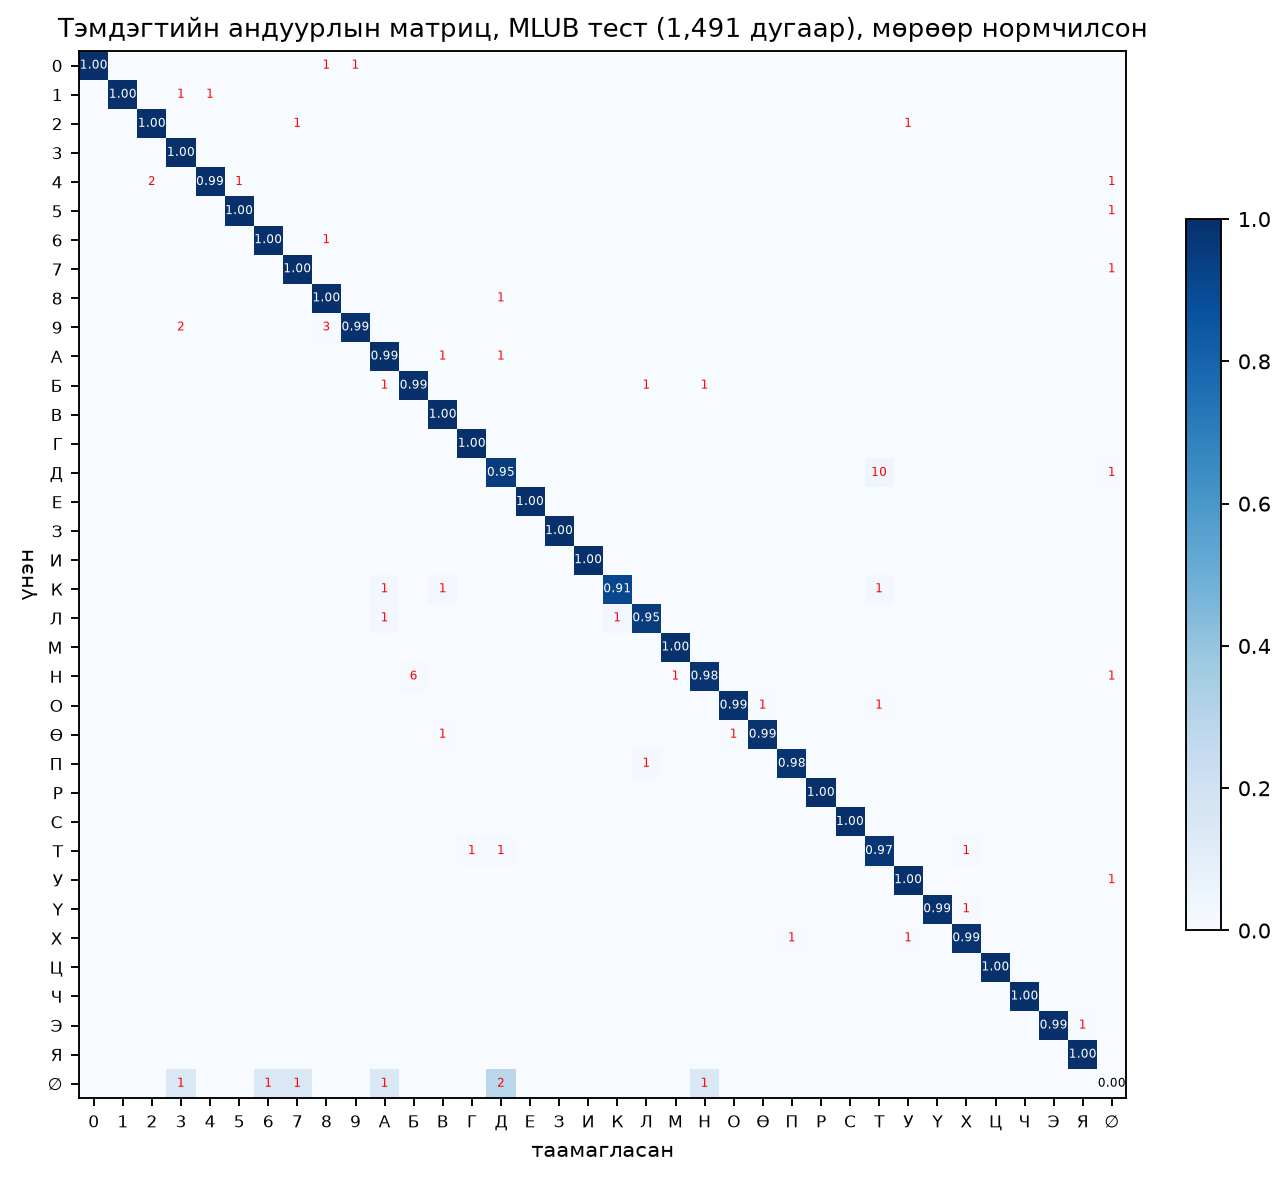
\includegraphics[width=0.92\textwidth]{confusion_mlub.png}
\caption{Тэмдэгтийн андуурлын матриц, MLUB тест (1\,491 дугаар, 10\,437 тэмдэгт), мөрөөр нормчилсон. Диагональд recall, диагоналиас гадуур алдааны тоо (улаан). $\varnothing$ нь орхигдсон (мөр) эсвэл илүү (багана) тэмдэгт.}\label{fig:cm}\end{figure}
\begin{figure}[H]\centering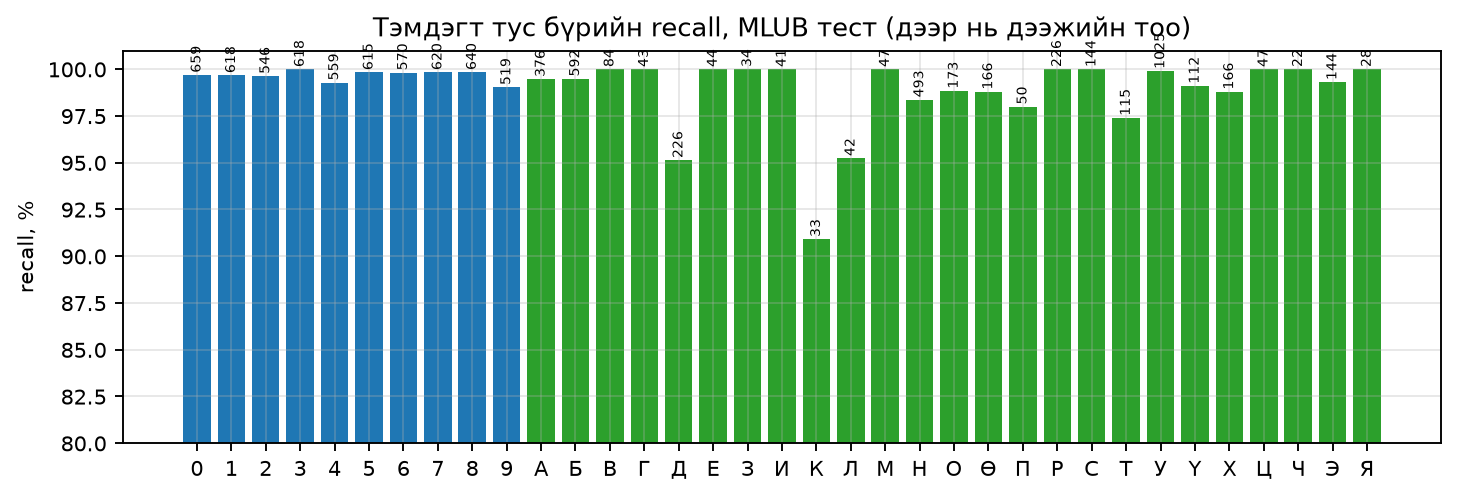
\includegraphics[width=\textwidth]{perchar_mlub.png}
\caption{Тэмдэгт тус бүрийн recall, MLUB тест; баганын дээр дээжийн тоо. Цэнхэр --- тоо, ногоон --- үсэг. Ховор серийн үсэг (К, Л, Д, Т) хамгийн бага.}\label{fig:perchar}\end{figure}
\begin{table}[H]\centering\caption{Хамгийн их андуурагдсан тэмдэгтийн хосууд, MLUB тест}\label{tab:conf}
\begin{tabular}{ccc|ccc}\toprule
Үнэн & Таамаг & Тоо & Үнэн & Таамаг & Тоо\\\midrule
Д & Т & 10 & Т & Х & 1\\
Н & Б & 6 & А & В & 1\\
9 & 8 & 3 & Т & Г & 1\\
9 & 3 & 2 & Ө & В & 1\\
4 & 2 & 2 & Э & Я & 1\\
$\varnothing$ & Д (илүү) & 2 & Ү & Х & 1\\\bottomrule
\end{tabular}\end{table}
\begin{figure}[H]\centering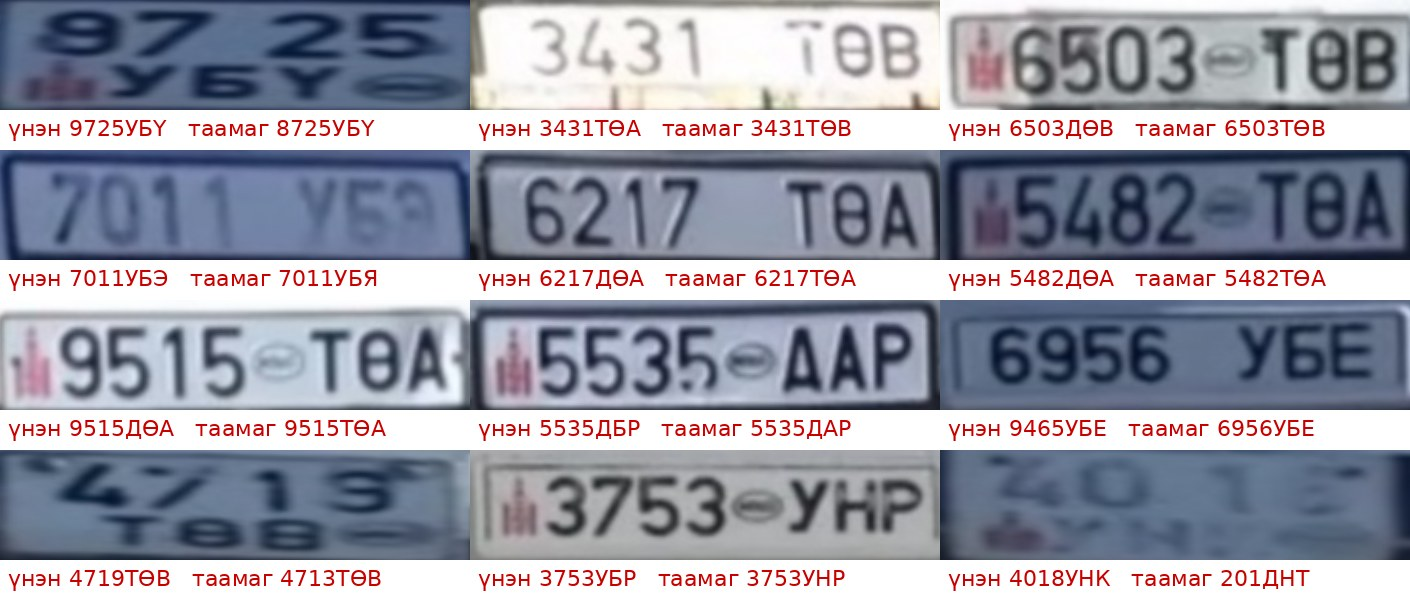
\includegraphics[width=\textwidth]{errors_mlub.jpg}
\caption{MLUB тест дээр буруу уншигдсан дугаарын жишээ (үнэн ба таамаг). Ихэнх нь бага нягтрал, бохирдол, хүчтэй шахалттай зураг дээрх нэг тэмдэгтийн андуурал.}\label{fig:errors}\end{figure}

\section{Төгсгөл хүртэлх үр дүн ба олон кадрын санал}
GitHub-ийн 18 бүтэн дүрстэй зураг (19 дугаар) дээр илрүүлэгч 18 дугаарыг IoU $\ge0.5$-аар олж (recall 94.7 хувь), 14-ийг яг зөв уншсан (73.7 хувь). Алдаа: нэг дугаар илрээгүй (\plate{2024УБЭ}); дөрөв нь сүүлийн үсгийн андуурал --- \plate{1537УНЛ}$\to$УНА, \plate{9494УБМ}$\to$УБИ, \plate{5947УБК}$\to$УБХ, \plate{3417УНТ}$\to$УНГ. Ижил 19 дугаарыг үнэн хайрцгаар өгөхөд 89.5 хувь байсан тул илрүүлэгчийн хайрцгийн зах, мөр хуваалтын зөрүү нэмэлт 2--3 алдаа үүсгэж байна. Зураг~\ref{fig:qual}-д төгсгөл хүртэлх жишээг үзүүлэв.
\begin{figure}[H]\centering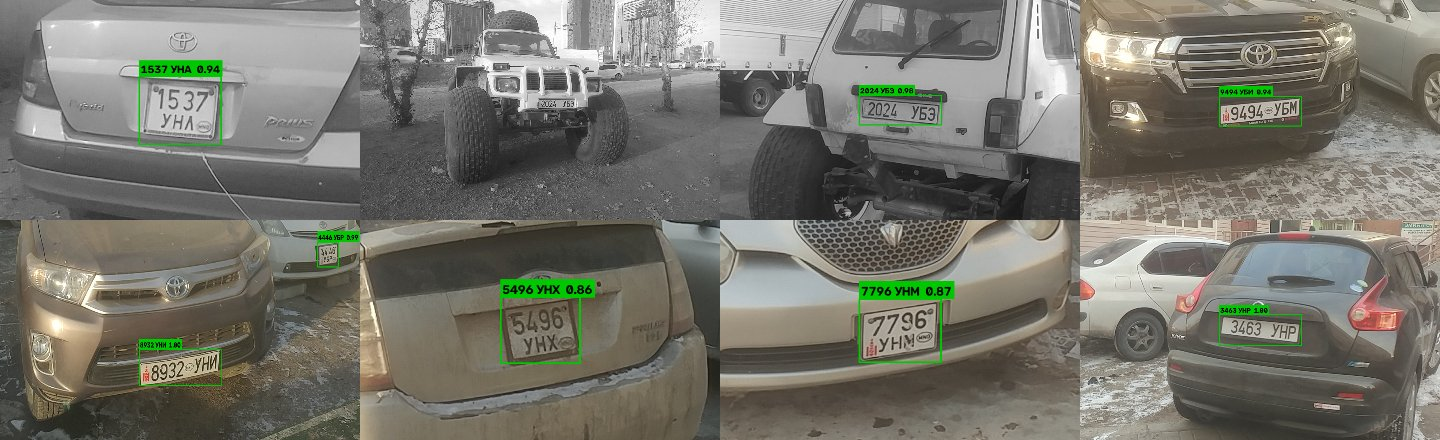
\includegraphics[width=\textwidth]{qualitative_github.jpg}
\caption{GitHub тестийн зураг дээрх төгсгөл хүртэлх үр дүн (ногоон: дүрэмд нийцсэн уншилт; шошго: дугаар ба уншигчийн итгэл). Нэг зурагт хоёр машин байхад хоёуланг нь олж уншсан жишээ.}\label{fig:qual}\end{figure}
Олон кадрын симуляцийн үр дүнг Зураг~\ref{fig:k}, Хүснэгт~\ref{tab:k}-д үзүүлэв. GitHub төгсгөл хүртэлх тестэд 3 кадрын санал 73.7-оос 78.9 хувь болгосон (нэг дугаар засагдсан), цаашид өсөөгүй; MLUB тайралтад санал 96.8 хувийг өөрчилсөнгүй. Учир нь симуляци нь нэг зургийн хувилбарууд дээр хийгдсэн тул алдаа \emph{системтэй} (бүх хувилбарт ижил тэмдэгт буруу) бөгөөд~\cite{wang2026mt}-д тэмдэглэснээр ийм алдааг санал засдаггүй. Бодит бичлэгт кадрууд өнцөг, зай, гэрлээр ялгаатай тул саналын ашиг тус илүү байхыг дараагийн хэсэг харуулна.
\begin{figure}[H]\centering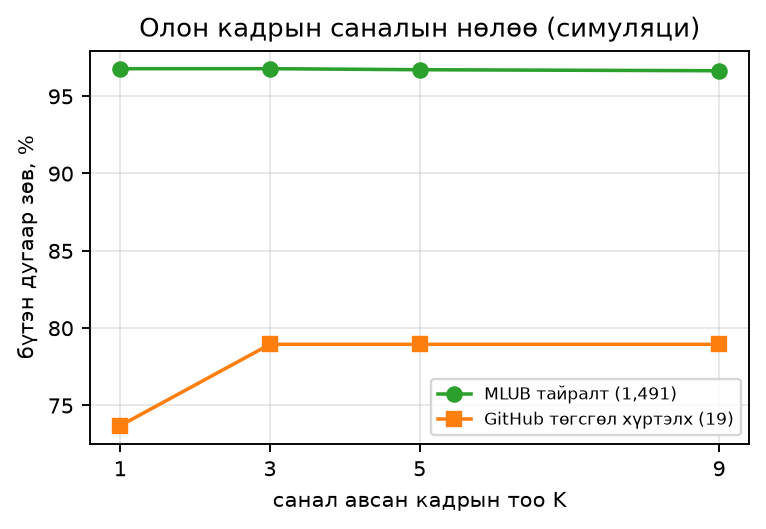
\includegraphics[width=0.6\textwidth]{multiframe_k.png}
\caption{Санал авсан кадрын тоо $K$-ийн нөлөө (симуляци).}\label{fig:k}\end{figure}
\begin{table}[H]\centering\caption{Олон кадрын саналын нөлөө, бүтэн дугаарын нарийвчлал (хувь), симуляцийн хувиргалт}\label{tab:k}
\begin{tabular}{lcccc}\toprule
Тест & $K=1$ & $K=3$ & $K=5$ & $K=9$\\\midrule
MLUB тайралт (1\,491) & 96.8 & 96.8 & 96.7 & 96.6\\
GitHub төгсгөл хүртэлх (19) & 73.7 & 78.9 & 78.9 & 78.9\\\bottomrule
\end{tabular}\end{table}

\section{Хугацааны хэмжилт}
Хүснэгт~\ref{tab:lat}, Зураг~\ref{fig:lat}-д 1920$\times$1080 кадрын боловсруулалтын хугацааг үзүүлэв. Нийт 7.3~мс (p95 9.8~мс) нь 100~мс зорилтоос 13 дахин бага бөгөөд 30~fps бичлэгийг бүх кадраар боловсруулах боломжтой. Анхны кадр 1.4~с (CUDA халаалт). GPU-гүй CPU дээр (16 цөм) 62~мс.
\begin{table}[H]\centering\caption{Нэг кадрын хугацаа, 1920$\times$1080, RTX 5080, FP16, 90 давталт (мс)}\label{tab:lat}
\begin{tabular}{lcccc}\toprule
Хэсэг & Дундаж & Медиан & p95 & Max\\\midrule
Илрүүлэгч (YOLO11n 640, урьд/дараах боловсруулалт орсон) & 4.0 & --- & --- & ---\\
Уншигч + дүрэм & 3.2 & --- & --- & ---\\
Нийт \texttt{process\_frame} & \textbf{7.3} & 7.0 & 9.8 & 12.8\\\bottomrule
\end{tabular}\end{table}
\begin{figure}[H]\centering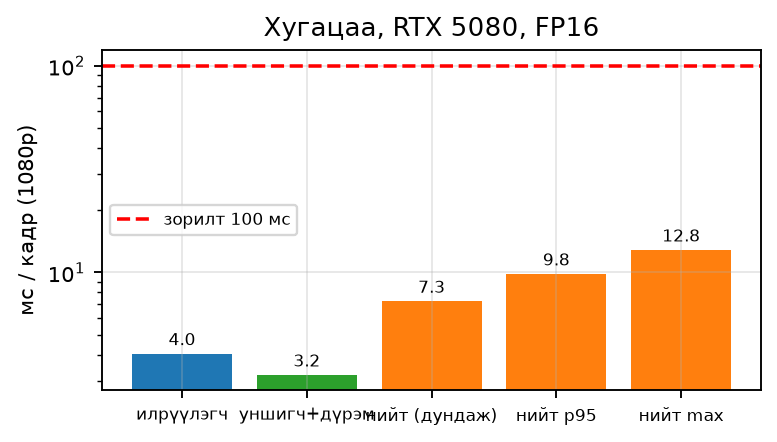
\includegraphics[width=0.6\textwidth]{latency.png}\caption{Хугацааны бүрэлдэхүүн (логарифм), 100~мс зорилттой харьцуулахад.}\label{fig:lat}\end{figure}

\section{Бичлэгийн туршилт}
Гурван бичлэгийг (хоёр нь гар утасны босоо 720$\times$1280, нэг нь хэвтээ 1280$\times$720, 30~fps) хоёр кадр тутамд нэгийг боловсруулж мөрдөлт, саналтайгаар ажиллуулав (Зураг~\ref{fig:video}, \ref{fig:tracks}). Нийт 29 мөр ($\ge3$ кадр) үүссэн. Хэвтээ, тогтвортой клипт 11 мөр бүгд дүрэмд нийцсэн дугаар өгч, margin 0.89--1.00, нэг кадрын санал нийцэл 0.30--1.00; нэг машин хоёр удаа орж ирэхэд ижил дугаар (\plate{1116 УНО}) гарсан. Гар утасны босоо клипт дугаар жижиг, хөдөлгөөний бүдэгтэй, налуу тул 18 мөрөөс 13 нь дүрэмд нийцсэн, 5 нь хог (хоёр зэргэлдээ дугаар нийлсэн зэрэг), санал нийцэл ихэвчлэн 0.3-аас бага. Үнэн шошго байхгүй тул энэ нь чанарын ажиглалт боловч margin ба санал нийцэл найдвартай/найдваргүй мөрийг тодорхой ялгаж байгаа нь хаалга нээх дүрэмд ашиглагдана.
\begin{figure}[H]\centering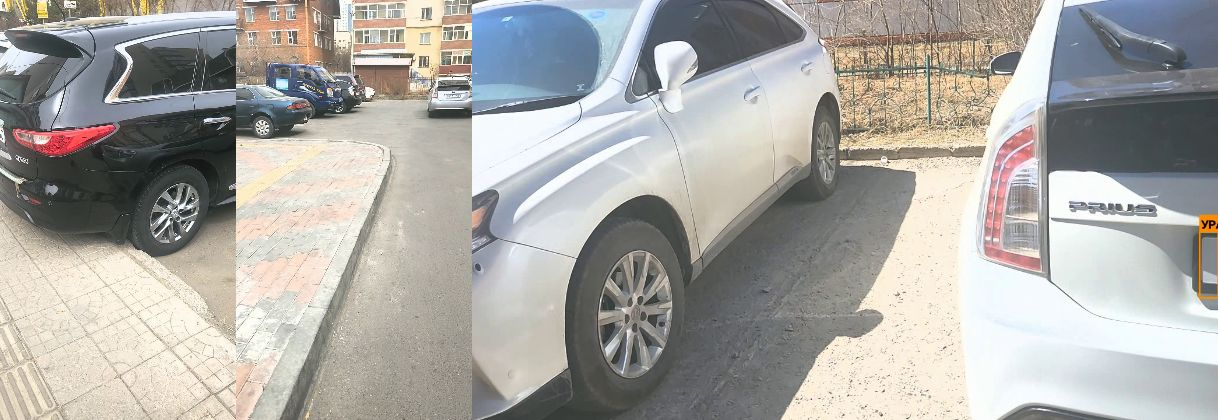
\includegraphics[width=\textwidth]{video_frames.jpg}
\caption{Гурван бичлэгийн тэмдэглэгээтэй кадр: мөр бүрийн санал нэгдсэн дугаар, итгэл, санал авсан кадрын тоо $n$.}\label{fig:video}\end{figure}
\begin{figure}[H]\centering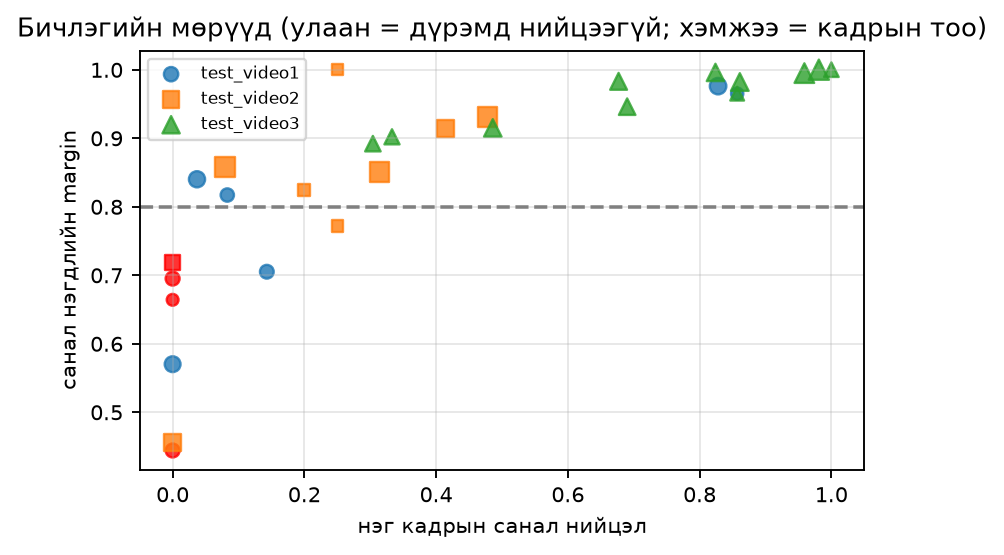
\includegraphics[width=0.7\textwidth]{video_tracks.png}
\caption{Бичлэгийн 29 мөр: нэг кадрын санал нийцэл ба санал нэгдлийн margin; улаан --- дүрэмд нийцээгүй; цэгийн хэмжээ --- кадрын тоо; тасархай шугам --- санал болгож буй margin босго 0.8.}\label{fig:tracks}\end{figure}

\section{Зорилттой харьцуулсан дүгнэлт}
\begin{table}[H]\centering\caption{Техникийн шаардлага ба хүрсэн үр дүн}\label{tab:targets}
\resizebox{\textwidth}{!}{\begin{tabular}{lccl}\toprule
Шаардлага & Зорилт & Хүрсэн & Байдал\\\midrule
Илрүүлэлт mAP$_{50}$ (монгол) & $\ge0.95$ & 0.992 & биелсэн\\
Бүтэн зөв уншилт, 1\,491 бодит дугаар & $\ge95$ хувь & 96.8 хувь (95 хувийн CI 96--98) & биелсэн\\
Хугацаа, 1080p кадр & $<100$~мс & 7.3~мс (p95 9.8) & биелсэн\\
Олон кадрын баталгаажуулалт & байх & IoU мөрдөлт + жинлэсэн санал & биелсэн\\
Төгсгөл хүртэлх, 19 бүтэн дүрстэй дугаар & $\ge95$ хувь & 73.7 / 78.9 хувь (CI 51--88) & биелээгүй\\
Туршилтын интерфэйс & байх & Gradio, зураг + бичлэг & биелсэн\\\bottomrule
\end{tabular}}\end{table}

\chapter{ХЭЛЭЛЦҮҮЛЭГ БА ЦААШДЫН АЖИЛ}
\section{Үр дүнгийн хэлэлцүүлэг}
\textbf{Илрүүлэгч.} Дугаарын геометр улс орноос үл хамаардаг тул 8\,823 олон улсын зураг дээр сургасан YOLO11n монгол дугаарыг шууд өндөр нарийвчлалтай олж (mAP$_{50}$ 0.98), 48 монгол зураг нэмэхэд хайрцгийн нарийвчлал (mAP$_{50\text{--}95}$ 0.69$\to$0.83) л сайжирсан. Энэ нь илрүүлэгчид монгол зураг харьцангуй цөөн байхад ч хангалттай, харин уншигчид бодит монгол өгөгдөл шийдвэрлэх ач холбогдолтой гэсэн дүгнэлтэд хүргэнэ.

\textbf{Бодит өгөгдлийн ач холбогдол.} Зөвхөн синтетик 42 хувь, 74 бодит мөр нэмэхэд 84 хувь, 7\,392 бодит тайралт нэмэхэд 97 хувь болсон нь (Хүснэгт~\ref{tab:ablation}) синтетик нь тэмдэгтийн хэлбэрийг зааж, бодит өгөгдөл домэйны онцлогийг заадаг гэсэн~\cite{jaderberg2014,ruder2022}-ын дүгнэлтийг давтаж байна. Монгол дугаарт текстээр шошголсон нээлттэй өгөгдөл байхгүй гэж үзэж байсан ч GitHub репо дотроос MLUB тэмцээний өгөгдөл олдсон нь ажлын чиглэлийг өөрчилсөн.

\textbf{Яагаад төгсгөл хүртэлх үр дүн доогуур вэ.} 1\,491 тайралт дээрх 96.8 хувь ба 19 бүтэн дүрстэй зураг дээрх 73.7 хувийн зөрүү таван шалтгаантай: (1) текстээр шошголсон бодит монгол өгөгдөл 7\,392 зураг, 5\,575 ялгаатай дугаар байгаа нь хятад (CCPD 300 мянга) зэрэгтэй харьцуулахад бага; (2) үсгийн тархалт тэнцвэргүй --- аймгийн кодоос болж У, Б, Н, А мянгаар байхад Л, К, М, И, Т, Г серийн үсэг 100--300 удаа л байгаа ба алдсан дөрвөн дугаар яг эдгээр үсэг дээр алдсан; (3) домэйн зөрүү --- MLUB замын камерын тайралт бол GitHub гар утасны бүтэн машины зураг, бохир, цастай, налуу, энэ домэйноос сургалтад 74 мөр л орсон; (4) илрүүлэгчийн хайрцаг үнэн хайрцгаас зөрөхөд мөр хуваалт өөрчлөгдөж 89.5-аас 77.8 хувь болдог; (5) 19 дугаар дээр нэг алдаа 5.3 нэгж хувь тул статистикийн хувьд хангалтгүй (95 хувийн Wilson интервал 51--88).

\textbf{Олон кадрын санал.} Симуляцид саналын ашиг бага (73.7$\to$78.9, MLUB-д өөрчлөлтгүй) байсан нь нэг зургийн хувилбарууд дээр алдаа системтэй учраас; бодит бичлэгт нэг кадрын санал нийцэл 0.3--0.8 байхад санал нэгдсэн дугаар тогтвортой гарч байгаа нь (Зураг~\ref{fig:tracks}) бодит нөхцөлд саналын ач холбогдол илүү гэдгийг харуулна. Margin ба нийцэл хоёр нь найдваргүй мөрийг ялгах тул хаалга нээх шийдвэрт заавал ашиглах хэрэгтэй.

\section{Хязгаарлалт}
\begin{itemize}[leftmargin=2em]
\item Бодит зураг бүгд өдрийн, өвлийн, гар утас эсвэл замын камерын; шөнө, бороо, гэрлийн гялбаа, хаалганы доод өнцгийг зөвхөн аугментаци дуурайсан.
\item Дипломат (улаан, ДК), цэргийн (ЦАБ), хилийн (ХЦА), чиргүүл, мотоциклийн дугаар байхгүй.
\item Хоёр мөрт хуваалт тогтмол 55/55 хувь; хүчтэй налуу (roll) үед мөр холилдоно.
\item MLUB хэлбэрийн шошго автомат (3 хувь орчим алдаатай); тестийн тоо үүгээр бага зэрэг дутуу үнэлэгдэнэ.
\item Төгсгөл хүртэлх тест 19 дугаартай; Roboflow-ийн 984 зураг API түлхүүргүй тул ашиглагдаагүй.
\item Бичлэгийн үр дүн үнэн шошгогүй тул чанарын.
\end{itemize}

\section{Явцын төлөв ба үлдсэн ажил}
\begin{table}[H]\centering\caption{Гүйцэтгэсэн ба үлдсэн ажил}\label{tab:todo}\small
\begin{tabular}{p{9cm}l}\toprule
Ажил & Төлөв\\\midrule
Судалгааны тойм, монгол дугаарын бүтэц, эх үүсвэрийн судалгаа & гүйцэтгэсэн\\
GitHub, HuggingFace, MLUB өгөгдөл бэлтгэх, текст сэргээх, давхцалгүй хуваалт & гүйцэтгэсэн\\
Синтетик дугаар үүсгэгч (90\,021 мөр) & гүйцэтгэсэн\\
YOLO11n хоёр үе шаттай сургалт, mAP$_{50}$ 0.992 & гүйцэтгэсэн\\
CRNN+CTC дөрвөн үе шаттай сургалт, 96.8 хувь & гүйцэтгэсэн\\
Дугаарын дүрэм, аймгийн код, олон кадрын жинлэсэн санал & гүйцэтгэсэн\\
Үнэлгээ, андуурлын шинжилгээ, хугацаа, бичлэгийн туршилт, Gradio интерфэйс & гүйцэтгэсэн\\
Roboflow 984 зураг нэмж илрүүлэгчийг дахин сургах & үлдсэн (API түлхүүр)\\
Зогсоолын камерын бодит бичлэг цуглуулж шошголох, домэйн тохируулга & үлдсэн\\
Синтетикт ховор үсгийг тэнцвэржүүлэх, test-time augmentation & үлдсэн\\
Сурсан мөр хуваалт эсвэл хоёр ангит илрүүлэгч & үлдсэн\\
CTC beam search + дүрмийн хязгаарлалттай декод & үлдсэн\\
ONNX/TensorRT, INT8 экспорт, edge төхөөрөмж дээр хэмжих & үлдсэн\\
Орох-гарах бүртгэл, засварлах зай $\le1$ тулгалт, хаалга нээх дүрэм, операторын засварын лог & үлдсэн\\\bottomrule
\end{tabular}\end{table}
Зогсоолын системд нэгтгэх санал: илрүүлэгчийг кадр бүрт, уншигчийг зөвхөн мөр үүссэн үед ажиллуулах; $\ge3$ кадр, дүрэмд нийцсэн, margin $\ge0.8$ үед хаалга нээх; хамгийн сайн тайралт, санал нэгдсэн дугаар, margin-ыг бүртгэлийн санд хадгалж гарах үед нээлттэй сессүүдтэй засварлах зай $\le1$-ээр тулгах; татгалзсан, бага margin-тай уншилт бүрийг оператор засаж, засвар нь дараагийн сургалтын өгөгдөл болно. Хэдэн зуун засварласан дугаар хуримтлагдсаны дараа уншигчийг дахин тохируулж, тестийн олонлогийг 500-аас дээш дугаар болгосноор 95 хувийн мэдэгдэл $\pm2$ нэгж хувийн интервалтай болно.

\chapter*{ДҮГНЭЛТ}\addcontentsline{toc}{chapter}{ДҮГНЭЛТ}\markboth{ДҮГНЭЛТ}{}
Энэ ажлаар зогсоолын системд зориулсан Монгол улсын дугаар таних хоёр шатлалт гүн сургалтын системийг бүтээж, нээлттэй эх үүсвэрээс олдсон бүх өгөгдлийг нэгтгэн үнэлгээний протокол тогтоов. Нээлттэй эх үүсвэрийн судалгаагаар GitHub-ийн 68 зураг (тэмдэгт бүрийн хайрцагтай), Roboflow-ийн 984 зураг (хайрцаг, API түлхүүр шаардлагатай), HuggingFace-ийн 8\,823 олон улсын зураг, GitHub репо дотор хадгалагдсан MLUB тэмцээний 7\,394 бодит дугаарын тайралт (текстээр) олдсон бөгөөд монгол дугаарын дизайныг дуурайсан 90\,021 синтетик мөр зураг үүсгэв. Тэмдэгтийн хайрцгаас дугаарын текст сэргээх, дугаарын давхцалгүй хуваалт, сунгасан хоёр мөрт дугаарын хэлбэрийг автоматаар шошголох аргуудыг боловсруулав.

YOLO11n илрүүлэгчийг олон улсын өгөгдөл дээр урьдчилан сургаж монгол зургаар нарийн тохируулахад монгол шалгалтын олонлог дээр mAP$_{50}=0.992$, mAP$_{50\text{--}95}=0.834$ хүрсэн нь зорилтыг хангав. Монгол кирилл 35 үсэг + 10 орны тэмдэгтийн олонлог дээр CRNN+CTC уншигчийг синтетик, GitHub, MLUB гэсэн дөрвөн үе шаттай сургахад 1\,491 бодит дугаар дээр 96.8 хувийн бүрэн зөв уншилт, 0.65 хувийн CER хүрч 95 хувийн зорилтыг давав; хоёр мөрт дугаар 98.4, нэг мөрт 95.8 хувь. Андуурлын шинжилгээгээр алдааны дийлэнх нь Д$\to$Т, Н$\to$Б зэрэг хэлбэрийн ойролцоо хос ба ховор серийн үсэг дээр төвлөрч байгааг тогтоов. Дугаарын дүрэм, 29 аймгийн код, итгэлээр жинлэсэн тэмдэгт тус бүрийн саналд суурилсан олон кадрын баталгаажуулалтыг хэрэгжүүлж, бүхэл урсгал нэг 1080p кадрыг 7.3~мс-д (p95 9.8~мс) боловсруулж 100~мс зорилтыг хангав. Бүтэн дүрстэй 19 дугаарын жижиг тест дээр төгсгөл хүртэлх нарийвчлал 73.7 хувь (9 кадрын саналаар 78.9 хувь) байгаа нь домэйн зөрүү, ховор үсэг, хайрцгийн зөрүүгээс үүдэлтэй бөгөөд зогсоолын камерын бодит өгөгдөл цуглуулах шаардлагыг тодорхой харуулав.

Дараагийн шатанд Roboflow өгөгдлийг нэмж илрүүлэгчийг дахин сургах, зогсоолын камерын бичлэг цуглуулж шошголох, ховор үсгийг тэнцвэржүүлэх, дүрмийн хязгаарлалттай декод, ONNX/TensorRT экспорт, орох-гарах бүртгэл ба хаалга нээх дүрмийг хэрэгжүүлж зогсоолын бүрэн систем болгон хөгжүүлнэ.

\begin{thebibliography}{99}\addcontentsline{toc}{chapter}{НОМ ЗҮЙ}\markboth{НОМ ЗҮЙ}{}
\bibitem{asianews2025} Asia News Network, ``Ulaanbaatar to restrict license plates for vehicles older than 10 years starting June 1,'' 2025. [Online]. Available: \url{https://asianews.network/}
\bibitem{wikimn} Wikipedia, ``Vehicle registration plates of Mongolia,'' accessed 14 Oct. 2026. [Online]. Available: \url{https://en.wikipedia.org/wiki/Vehicle_registration_plates_of_Mongolia}
\bibitem{dierkes2019} J. Dierkes, ``Special license plates,'' Mongolia Focus (Univ. of British Columbia), Aug. 2019. [Online]. Available: \url{https://mongoliafocus.com/2019/08/official_cars/}
\bibitem{laroca2018} R. Laroca, E. Severo, L. A. Zanlorensi, L. S. Oliveira, G. R. Gon\c{c}alves, W. R. Schwartz, and D. Menotti, ``A robust real-time automatic license plate recognition based on the YOLO detector,'' in \emph{Proc. Int. Joint Conf. Neural Networks (IJCNN)}, 2018, pp. 1--10.
\bibitem{wang2026mt} Q. Wang \emph{et al.}, ``A multi-task deep learning framework for real-time intelligent video surveillance with temporal event validation,'' arXiv:2607.03131, 2026.
\bibitem{pham2023ctsm} H. Pham \emph{et al.}, ``Character time-series matching for robust license plate recognition,'' arXiv:2307.11336, 2023.
\bibitem{shi2017crnn} B. Shi, X. Bai, and C. Yao, ``An end-to-end trainable neural network for image-based sequence recognition and its application to scene text recognition,'' \emph{IEEE Trans. Pattern Anal. Mach. Intell.}, vol. 39, no. 11, pp. 2298--2304, 2017.
\bibitem{graves2006ctc} A. Graves, S. Fern\'andez, F. Gomez, and J. Schmidhuber, ``Connectionist temporal classification: Labelling unsegmented sequence data with recurrent neural networks,'' in \emph{Proc. 23rd Int. Conf. Machine Learning (ICML)}, 2006, pp. 369--376.
\bibitem{ppocr} Y. Du \emph{et al.}, ``PP-OCR: A practical ultra lightweight OCR system,'' arXiv:2009.09941, 2020; PaddleOCR, \url{https://github.com/PaddlePaddle/PaddleOCR}.
\bibitem{yolo11} G. Jocher and J. Qiu, ``Ultralytics YOLO11,'' 2024. [Online]. Available: \url{https://github.com/ultralytics/ultralytics}
\bibitem{morse2025} Morse Tech Lab, ``yolov11-license-plate-detection,'' Hugging Face model card, 2025.
\bibitem{jaderberg2014} M. Jaderberg, K. Simonyan, A. Vedaldi, and A. Zisserman, ``Synthetic data and artificial neural networks for natural scene text recognition,'' in \emph{NIPS Deep Learning Workshop}, 2014.
\bibitem{ruder2022} A. Ruder \emph{et al.}, ``Synthesizing annotated image and video data using a rendering-based pipeline for improved license plate recognition,'' arXiv:2209.14448, 2022.
\bibitem{ccpd} Z. Xu \emph{et al.}, ``Towards end-to-end license plate detection and recognition: A large dataset and baseline (CCPD),'' in \emph{Proc. ECCV}, 2018.
\bibitem{ufpr} R. Laroca \emph{et al.}, ``UFPR-ALPR dataset,'' 2018. [Online]. Available: \url{https://github.com/raysonlaroca/ufpr-alpr-dataset}
\bibitem{gumbernator} gumbernator, ``Mongolian-ALPR: Mongolian automated license plate recognition,'' GitHub repository (fork: algorithm-developer/Mongolian-ALPR), accessed 14 Oct. 2026. [Online]. Available: \url{https://github.com/gumbernator/Mongolian-ALPR}
\bibitem{tsund} Tsundgerhen, ``mongolian\_licence\_plate: YOLOv8-based Mongolian license plate detection,'' GitHub repository, 2025. [Online]. Available: \url{https://github.com/Tsundgerhen/mongolian_licence_plate}
\bibitem{narangoo} narangoo9, ``Mongolian-License-Plate-Recognition-System,'' GitHub repository, 2026.
\bibitem{roboflowmn} Computer Vision (workspace), ``mongolian plate dataset,'' Roboflow Universe, Apr. 2025. [Online]. Available: \url{https://universe.roboflow.com/computer-vision-m1xzb/mongolian-plate}
\bibitem{keremberke} keremberke, ``license-plate-object-detection (Roboflow Vehicle Registration Plates, 8,823 images),'' Hugging Face Datasets, 2023.
\bibitem{paszke2019} A. Paszke \emph{et al.}, ``PyTorch: An imperative style, high-performance deep learning library,'' in \emph{Advances in Neural Information Processing Systems 32}, 2019.
\end{thebibliography}

\appendix
\chapter{АЙМАГ, ХОТЫН КОДЫН ХҮСНЭГТ}\label{app:regions}
\begin{table}[H]\centering\caption{Дугаарын эхний хоёр үсгийн бүртгэлийн бүсийн код (\texttt{mn\_alpr/plate\_rules.py})}\small
\begin{tabular}{ll|ll|ll}\toprule
Код & Бүс & Код & Бүс & Код & Бүс\\\midrule
АР & Архангай & ДУ & Дундговь & СҮ & Сүхбаатар\\
БН & Баянхонгор & ОР & Орхон & СБ & Сүхбаатар хот\\
БР & Багануур (УБ) & ХЭ & Хэнтий & ТӨ & Төв\\
БӨ & Баян-Өлгий & ХО & Ховд & УБ, УН, УА, УЕ, УК & Улаанбаатар\\
БУ & Булган & ХӨ & Хөвсгөл & УВ & Увс\\
ГА & Говь-Алтай & НА & Налайх (УБ) & ЗА & Завхан\\
ГС & Говьсүмбэр & ӨМ & Өмнөговь & ДК & Дипломат\\
ДА & Дархан-Уул & ӨВ & Өвөрхангай & ЦА & Цэрэг\\
ДГ & Дорноговь & СЭ & Сэлэнгэ & ХЦ & Хилийн цэрэг\\
ДО & Дорнод & & & &\\\bottomrule
\end{tabular}\end{table}

\chapter{ТЭМДЭГТ ТУС БҮРИЙН ДЭЛГЭРЭНГҮЙ ҮР ДҮН}\label{app:perchar}
\begin{table}[H]\centering\caption{MLUB тест (1\,491 дугаар): тэмдэгт тус бүрийн дээжийн тоо ба recall}\small
\begin{tabular}{lrr|lrr|lrr}\toprule
Тэмдэгт & Дээж & Recall & Тэмдэгт & Дээж & Recall & Тэмдэгт & Дээж & Recall\\\midrule
0 & 659 & 99.7 & В & 84 & 100.0 & П & 50 & 98.0\\
1 & 618 & 99.7 & Г & 43 & 100.0 & Р & 226 & 100.0\\
2 & 546 & 99.6 & Д & 226 & 95.1 & С & 144 & 100.0\\
3 & 618 & 100.0 & Е & 44 & 100.0 & Т & 115 & 97.4\\
4 & 559 & 99.3 & З & 34 & 100.0 & У & 1025 & 99.9\\
5 & 615 & 99.8 & И & 41 & 100.0 & Ү & 112 & 99.1\\
6 & 570 & 99.8 & К & 33 & 90.9 & Х & 166 & 98.8\\
7 & 620 & 99.8 & Л & 42 & 95.2 & Ц & 47 & 100.0\\
8 & 640 & 99.8 & М & 47 & 100.0 & Ч & 22 & 100.0\\
9 & 519 & 99.0 & Н & 493 & 98.4 & Э & 144 & 99.3\\
А & 376 & 99.5 & О & 173 & 98.8 & Я & 28 & 100.0\\
Б & 592 & 99.5 & Ө & 166 & 98.8 &  & & \\
\bottomrule\end{tabular}\end{table}

\chapter{СУРГАЛТЫН ТОХИРГООНЫ ФАЙЛ}\label{app:config}
\section{Илрүүлэгчийн B үеийн өгөгдлийн тохиргоо}
\begin{lstlisting}[language=,caption={configs/det\_stageB.yaml}]
path: data/det
train: [hf_plates/images/train, github_rep/images/train]
val: github/images/val
names:
  0: plate
\end{lstlisting}
\section{Сургалт, үнэлгээний командууд}
\begin{lstlisting}[language=bash,caption={Бүрэн дахин сургах дараалал}]
python scripts/prepare_github_data.py
python scripts/prepare_hf_data.py
python scripts/synth_plates.py --n 60000
python scripts/train_det.py --epochsA 25 --epochsB 60
python scripts/train_rec.py --real_rep 0 --epochs 10 --out runs/rec/synth_only
python scripts/train_rec.py --resume runs/rec/synth_only/best.pt --epochs 6 \
    --lr 3e-4 --out runs/rec/crnn
cp runs/rec/crnn/best.pt models/plate_rec_crnn.pt
python scripts/prepare_mlub_data.py
python scripts/train_rec.py --resume models/plate_rec_crnn.pt \
    --real data/rec/real_mlub data/rec/real_github --real_rep 40 \
    --epochs 8 --lr 5e-4 --out runs/rec/crnn_mlub_r1
cp runs/rec/crnn_mlub_r1/best.pt models/plate_rec_crnn.pt
python scripts/prepare_mlub_data.py      # re-label layouts
python scripts/train_rec.py --resume models/plate_rec_crnn.pt \
    --real data/rec/real_mlub data/rec/real_github --real_rep 40 \
    --min_rep 3 --epochs 20 --lr 5e-4 --out runs/rec/crnn_mlub
cp runs/rec/crnn_mlub/best.pt models/plate_rec_crnn.pt
python scripts/eval_pipeline.py --frames 9
python scripts/run_videos.py
python app/gradio_app.py
\end{lstlisting}

\chapter{КОДЫН ХЭРЭГЖҮҮЛЭЛТ}\label{app:code}
\section{CRNN загвар}
\begin{lstlisting}[language=Python,caption={mn\_alpr/crnn.py: CRNN (residual CNN + BiLSTM + CTC head)}]
class CRNN(nn.Module):
    def __init__(self, num_classes=NUM_CLASSES, hidden=192):
        super().__init__()
        self.stem = nn.Sequential(nn.Conv2d(3, 32, 3, 1, 1, bias=False),
                                  nn.BatchNorm2d(32), nn.ReLU(inplace=True))
        self.layers = nn.Sequential(
            ConvBlock(32, 64, (2, 2)),    # 24 x 96
            ConvBlock(64, 128, (2, 2)),   # 12 x 48
            ConvBlock(128, 128),
            ConvBlock(128, 256, (2, 1)),  # 6 x 48
            ConvBlock(256, 256),
            ConvBlock(256, 384, (2, 1)),  # 3 x 48
            ConvBlock(384, 384))
        self.pool = nn.AdaptiveAvgPool2d((1, None))
        self.rnn = nn.LSTM(384, hidden, num_layers=2, bidirectional=True,
                           batch_first=True, dropout=0.1)
        self.fc = nn.Linear(2 * hidden, num_classes)

    def forward(self, x):                  # x: B,3,48,192
        f = self.layers(self.stem(x))      # B,384,3,48
        f = self.pool(f).squeeze(2).permute(0, 2, 1)   # B,T=48,C
        f, _ = self.rnn(f)
        return self.fc(f)                  # B,T,num_classes
\end{lstlisting}
\section{Дугаарын дүрэм ба магадлалын оноо}
\begin{lstlisting}[language=Python,caption={mn\_alpr/plate\_rules.py (хэсэгчлэн)}]
PLATE_RE = re.compile(r"^(\d{4})([%s]{3})$" % LETTERS)
LATIN2CYR = str.maketrans("ABEKMHOPCTYX", "ABEKMHOPCTYX")  # Latin -> Cyrillic look-alikes (second string is Cyrillic)

def normalize(text):
    t = text.upper().translate(LATIN2CYR)
    return re.sub(r"[^0-9%s]" % LETTERS, "", t)

def plausibility(text):
    m = PLATE_RE.match(normalize(text))
    if not m: return 0.0
    s = 0.6
    if m.group(2)[:2] in REGION_CODES: s += 0.3
    if m.group(2)[2] in SERIAL_LETTERS: s += 0.1
    return s
\end{lstlisting}
\section{Олон кадрын жинлэсэн санал}
\begin{lstlisting}[language=Python,caption={mn\_alpr/pipeline.py: PlateTrack}]
class PlateTrack:
    def add(self, text, conf, box):
        self.box = box; self.n += 1; self.missed = 0
        if not text: return
        w = conf * (0.5 + PR.plausibility(text))   # confidence x grammar prior
        self.votes.setdefault(len(text), [dict() for _ in range(len(text))])
        for i, ch in enumerate(text):
            self.votes[len(text)][i][ch] = self.votes[len(text)][i].get(ch, 0.0) + w

    def consensus(self):
        L = max(self.votes, key=lambda l: sum(sum(d.values()) for d in self.votes[l])
                * (1.3 if l == 7 else 1.0))
        chars, margins = [], []
        for d in self.votes[L]:
            items = sorted(d.items(), key=lambda kv: -kv[1]); tot = sum(d.values())
            chars.append(items[0][0]); margins.append(items[0][1] / tot)
        return "".join(chars), float(np.mean(margins)), self.n
\end{lstlisting}
\section{Хэлбэр тодорхойлох ба мөр хуваах}
\begin{lstlisting}[language=Python,caption={mn\_alpr/pipeline.py: Recognizer.read\_plate}]
def read_plate(self, crop):
    h, w = crop.shape[:2]
    if w / max(1, h) < TWO_LINE_AR:            # 1.8 -> two-line plate
        top = crop[: int(h * 0.55)]; bot = crop[int(h * 0.45):]
        t, c = self.read_lines([top, bot])
        return PR.normalize(t[0] + t[1]), float(min(c)), "two-line"
    t, c = self.read_lines([crop])
    return PR.normalize(t[0]), float(c[0]), "single-line"
\end{lstlisting}

\end{document}
